\section{Step 1: Design a basic disc storage system}
\subsection{Disc Data Structure}
In \texttt{step1/include/disc.h}, there is a struct called \texttt{Disc} which 
simulates a real disc. Its structure is as follows.

\begin{lstlisting}[language=C]
typedef struct {
    int _numCylinder;               // * # of cylinders
    int _numSectorPerCylinder;      // * # of sector per cylinder
    int _fd;                        // * file descriptor
    int _prev_cylinder;             // * previous cylinder
    double _trackDelay;             // * time delay moving between tracks
    char* _file;                    // * file name
    char* _discfile;                // * disc file mapped to the current file
    FILE* _fp;                      // * file pointer
} Disc;

\end{lstlisting}

I will expand on the purpose of each field in the following list.

\begin{itemize}
    \item \texttt{_numCylinder} is used to store the number of cylinders in the disc.
    \item \texttt{_numSectorPerCylinder} is used to store the number of sectors in each cylinder. Together
    with \texttt{_numCylinder}, they are the basic parameters of the disc which defines the size.
    \item \texttt{_fd} is the file descriptor of the file provided by command line input.
    \item \texttt{_prev\_cylinder} is used to store the previous cylinder number. This is used to calculate
    the time delay when moving between tracks.
    \item \texttt{_trackDelay} is used to store the time delay when moving between tracks. 
    \item \texttt{_file} is used to store the file name provided by command line input.
    \item \texttt{_discfile} is used to store the disc file name which is mapped to the current file. It is
    a key point in the design. We change the read/write operation on the disc to memory copy and write
   operation on the disc file. 
   \item \texttt{_fp} is actually a \textbf{redundant} variable. It is intended to store the file pointer of the
    given file, but it is not used in the final implementation.
\end{itemize}

\subsection{Operation Function}
In this subsection, i will expand on the design of the operation functions of the disc. They are declared in 
\texttt{step1/include/disc.h} and defined in \texttt{step1/src/disc.c}.

\subsubsection{constructor function}
This function has prototype \texttt{void constructor(int numCylinder, int numSectorPer\\Cylinder, double trackDelay, char* file, Disc* disc);}
. It initialize a disc with basic background info, namely assigning the parameters to the corresponding fields of the disc struct.
We initialize the \texttt{_prev_cylinder} to be 0, and \texttt{_fd} to be the return value of 
\texttt{open(disc->_file, O_RDWR | O_CREAT, S_IRUSR | S_IWUSR | S_IRGRP | S_IROTH)}. The reason why we need \texttt{O\_CREAT etc} 
is that we need to make sure the file can be open or created with \textbf{WRITE Permission}.
We suppose that a block has 256 bytes, thus calculating the total size of the disc.
And then we stretch the file to the size of the disc with \texttt{lseek()} function.
Finally, we map the file to the memory with \texttt{mmap()} function, and assign its return value to \texttt{_discfile}.

If the return value of \texttt{open(), lseek() and mmap()} is abnormal, the program will perror and exit.

Full code of this part is as follows.

\begin{lstlisting}[language=C]
    void constructor(int numCylinder, int numSectorPerCylinder, double trackDelay, char* file, Disc* disc) {
        disc->_file = file;
        disc->_numCylinder = numCylinder;
        disc->_numSectorPerCylinder = numSectorPerCylinder;
        disc->_trackDelay = trackDelay;
        disc->_prev_cylinder = 0;
        // * Make sure O_CREAT can create file with write permission.
        disc->_fd = open(disc->_file, O_RDWR | O_CREAT, S_IRUSR | S_IWUSR | S_IRGRP | S_IROTH);
        if (disc->_fd == -1) {
            printf("Error in creating or opening file %s. Check again.", disc->_file);
            exit(-1);
        }
        long FILESIZE = BLOCK_SIZE * disc->_numCylinder * disc->_numSectorPerCylinder;
        int result = lseek(disc->_fd, FILESIZE - 1, SEEK_SET);
        if (result == -1) {
            perror("Error calling lseek() to stretch the file.");
            close(disc->_fd);
            exit(-1);
        }
        result = write(disc->_fd, "", 1);
        if (result != 1) {
            perror("Error writing last byte of the file.");
            close(disc->_fd);
            exit(-1);
        }
        disc->_discfile = (char*) mmap(NULL, FILESIZE, PROT_READ | PROT_WRITE, MAP_SHARED, disc->_fd, 0);
        if (disc->_discfile == MAP_FAILED) {
            close(disc->_fd);
            perror("Error: Could not map file.");
            exit(-1);
        }
    }
\end{lstlisting}

\subsubsection{destructor function}
This function has prototype \texttt{void decontructor(Disc* disc)}.
The major task of this function is to unmap the file from the memory and close the file descriptor.

The code is as follows.

\begin{lstlisting}[language=C]
    void decontructor(Disc* disc) {
    // free(disc->_file);
    int result = munmap(disc->_discfile, BLOCK_SIZE * disc->_numCylinder * disc->_numSectorPerCylinder);
    if (result == -1) {
        perror("Error when unmmaping the memory space allocated to the file.");
        close(disc->_fd);
        exit(-1);
    }
    result = close(disc->_fd);
    if (result == -1) {
        perror("Error when closing the file descriptor.");
        exit(-1);
    }
    printf("\n\nDeconstructor successfully.\n");
}
\end{lstlisting}

\subsubsection{parseCmdInput function}
This is the major function to deal with user input.
It parses user command line input and calls corresponding detailed function to handle the operation.
It has the prototype \texttt{void parseCmdInput(Disc* disc, char* cmd)}.

In the body of the function, we first separate \texttt{cmd} into token by \texttt{space, [backslash]n}

\texttt{[backslash]r}. The latter one 
is the linux newline character. We count the length of input tokens simultaneously. 
Then, we switch case on the length, if length is one, the \texttt{cmd} must be \texttt{I}, so we check 
the first token, if it is \texttt{I}, we call \texttt{queryOp()} to deal with this query, otherwise, we exit with error message.
So is the case for length 3 and 5. They respectively mush be \texttt{R} and \texttt{W}. We check whether 
the first token is \texttt{R} or \texttt{W}, and then call \texttt{readOp()} or \texttt{writeOp()} to deal with the operation.
Still, we exit with error message if the first token is not \texttt{R} or \texttt{W}.

It is worth noting that i add two additional functions/commands, they are \texttt{R index} and \texttt{W index len data}.
It is important for the second part because the file system prefers using the block index, rather than the cylinder and sector index.
So disc side can provide a helper function to hide the conversion for the file system server. They are respectively \texttt{readOp\_client()} and \texttt{writeOp\_client()}.
Consequently, if the length is 2 or 4, we check the first token, if it is \texttt{R} or \texttt{W}, we call \texttt{readOp\_client()} or \texttt{writeOp\_client()} to deal with the operation.
Otherwise, we exit with error message.

The code is quite long, i choose a small snippet to show the logic. See below.

\begin{lstlisting}
    void parseCmdInput(Disc* disc, char* cmd) {
    char* token = strtok(cmd, " \n\r");
    char** argv = malloc(MAX_ARGS * sizeof(char*));
    int i = 0;
    while (token != NULL) {
        argv[i++] = token;
        token = strtok(NULL, " \n\r");
    }
    argv[i] = NULL;
    switch (i) {
        // * In parsing, we need to make sure int type arguments do have its int type value
        // * Whether the value is valid will be left to specific dealing function.
        case 1:
            if (strcmp(argv[0], "I") != 0) {
                // printf("strcmp is %d\n", strcmp(argv[0], "I"));
                perror("Wrong types of command of length 1. Please input 'I'.");
                free(argv);
                exit(-1);
            } else {
                queryOp(disc);
            }
            break;

        ...
    }
    ...
}
\end{lstlisting}

\subsubsection{queryOp function}
This is the function that handles \texttt{I} command. It has the prototype \texttt{void queryOp(Disc* disc)}. And it 
prints the \texttt{_numCylinder, _numSectorPerCylinder} of the disc provided. 

\subsubsection{readOp function}
This is the function that handles \texttt{R} command. It has the prototype \texttt{void readOp(Disc* disc, int cylinderId, int sectorId)}.
It first determines whether the input disc sector is valid. If not, it will print \texttt{No} as required.
Otherwise, it copies the data at given index of the disc into a buffer and concatenate it after \texttt{Yes} and then prints out.
We then use \texttt{usleep()} to simulate the time delay when moving between tracks. And we modify the \texttt{_prev_cylinder} to the current cylinder.

The code is as follows.

\begin{lstlisting}[language=C]
    void readOp(Disc* disc, int cylinderId, int sectorId) {
        char buf[BLOCK_SIZE + 1];
        memset(buf, 0, BLOCK_SIZE + 1);
        if (cylinderID < 0 || cylinderID >= disc->_numCylinder || sectorID < 0 || sectorID >= disc->_numSectorPerCylinder) {
            printf("No\n");
            return;
        }
        memcpy(buf, &disc->_discfile[BLOCK_SIZE * (cylinderID * disc->_numSectorPerCylinder + sectorID)], BLOCK_SIZE);
        usleep(disc->_trackDelay * abs(disc->_prev_cylinder - cylinderID));
        disc->_prev_cylinder = cylinderID;
        printf("Yes %s\n", buf);
}
\end{lstlisting}

Then we show the code of \texttt{readOp\_client()} function. You can easily check that it is a simple syntax sugar.

\begin{lstlisting}[language=C]
void readOp_client(Disc* disc, int blockID) {
    readOp(disc, blockID / disc->_numSectorPerCylinder, blockID % disc->_numSectorPerCylinder);
}
\end{lstlisting}

\subsubsection{writeOp function}
This is the function that handles \texttt{W} command. It has the prototype \texttt{void writeOp(Disc* disc, int cylinderId, int sectorId, int len, char* data)}.
It first determines whether the input disc sector is valid. If not, it will print \texttt{No} as required.
Otherwise, it copies the \texttt{len} long \texttt{data} to the given index of the disc. And then prints out \texttt{Yes}.
Specifically, if the length of the data is less than the block size, we fill the rest with 0.
Likewise, we use \texttt{usleep()} to simulate the time delay when moving between tracks. And we modify the \texttt{_prev_cylinder} to the current cylinder.

The code is as follows.

\begin{lstlisting}[language=C]
void writeOp(Disc* disc, int cylinderID, int sectorID, int len, char* data) {
    if (cylinderID < 0 || cylinderID >= disc->_numCylinder || sectorID < 0 || sectorID >= disc->_numSectorPerCylinder || len < 0 || len > BLOCK_SIZE) {
        printf("No\n");
        return;
    }
    memcpy(&disc->_discfile[BLOCK_SIZE * (cylinderID * disc->_numSectorPerCylinder + sectorID)], data, len);
    if (len < BLOCK_SIZE) {
        memset(&disc->_discfile[BLOCK_SIZE * (cylinderID * disc->_numSectorPerCylinder + sectorID) + len], 0, BLOCK_SIZE - len);
    }
    usleep(disc->_trackDelay * abs(disc->_prev_cylinder - cylinderID));
    disc->_prev_cylinder = cylinderID;
    printf("Yes\n");
}
\end{lstlisting}

Then we show the code of \texttt{writeOp\_client()} function. You can easily check that it is a simple syntax sugar.

\begin{lstlisting}[language=C]
    void writeOp_client(Disc* disc, int blockID, int len, char* data) {
        writeOp(disc, blockID / disc->_numSectorPerCylinder, blockID % disc->_numSectorPerCylinder, len, data);
    }
\end{lstlisting}

\subsection{BDS Design}
BDS is the abbreviation of Basic Disc Server, it has two main features. 
First, it has a global \texttt{Disc} type variable, and will be initialized 
based on command line input, which is stored in \texttt{argv}. Second, it uses 
socket to listen and accept client connection. Once connected, it will fork a child process to deal with the client request.
We add another special case to signal the end of the connection, which is \texttt{Q}.
Once received, the child process will close the connection file descriptor and exit. To exit the BDS program, 
i will use \texttt{Ctrl + C} to send a signal to the parent process, and set the signal handler to deal with the signal.
The signal handler will call \texttt{decontructor()} to free the memory and close the file descriptor and then exit.

Because we use write redirection to the client file descriptor, we need to manually flush the stdout buffer to make sure the client can receive the message in time. (printf may be cached in the buffer)

So the main framework of the BDS is as follows.

\begin{lstlisting}[language=C]
// Header files
// Macro definition

Disc d;

void sig_handler(int signo) {
    if (signo == SIGINT) {
        decontructor(&d);
        exit(EXIT_SUCCESS);
    }
}

int main(int argc, char** argv) {
    signal(SIGINT, sig_handler);
    
    // Socket initialization
    ... 
    constructor(atoi(argv[2]), atoi(argv[3]), strtod(argv[4], NULL), argv[1], &d);
    
    while (1) {
        // Socket Connection
        ... 
        if (pid == 0) {
            close(sockfd);
            char input[MAX_INPUT];
            dup2(clientfd, 1);
            dup2(clientfd, 2);
            while (1) {
                memset(input, 0, sizeof(input));
                int n = read(clientfd, input, sizeof(input));
                if (strcmp(strtok(input, "\n\r"), "Q") == 0) {
                    write(clientfd, "Goodbye.\n", 9);
                    break;
                }
                parseCmdInput(&d, input);
                // * Manually flush stdout buffer
                fflush(stdout);
            }
            close(clientfd);
            exit(EXIT_SUCCESS);
        } else {
            close(clientfd);
        }
    }
}    
\end{lstlisting}

\subsection{BDC\_CLI and BDC\_RANDOM Design}
\label{sec:bdc}
BDC\_CLI and BDC\_RANDOM are two client programs to interact with the BDS. They are quite similar, 
the only difference is that the former takes user input while the latter one generates random input.

We first expand on the features of BDC\_CLI. It will first connect to the server based on 
the command line input using socket, and then it will run an infinite loop to take user input via \texttt{fgets()} and then send it to the server via \texttt{send()}, then receive the response from the server via \texttt{recv()} and print it out.
Note the special case that when the user input is \texttt{Q}, the client will send it to the server and then exit.

The main framework of BDC\_CLI is as follows.

\begin{lstlisting}[language=C]
// Header files
// Macro definition

int main(int argc, char** argv) {
    // Socket initialization and connection
    ...
    printf("Connected to the server.\n");
    char cmd[MAX_INPUT];
    char response[MAX_RESPONSE];

    while (1) {
        printf("Disc Query: ");
        memset(cmd, 0, MAX_INPUT);
        fgets(cmd, MAX_INPUT, stdin);
        if (send(sockfd, cmd, sizeof(cmd), 0) < 0) {
            perror("Send failed");
            exit(-1);
        }
        memset(response, 0, sizeof(response)); 
        int recv_len = recv(sockfd, response, sizeof(response) - 1, 0); 
        if (recv_len < 0) {
            perror("Receive failed");
            exit(-1);
        } else if (recv_len == 0) {
            break;
        }
        printf("Result: %s\n", response);
        fflush(stdout);
        if (strcmp(strtok(cmd, " \n\r"), "Q") == 0) {
            break;
        }
    }

}
\end{lstlisting}

Then we expand on the features of BDC\_RANDOM. We first manually send the \texttt{I} command to the server to get the disc information. Then we randomly select a command from \texttt{R} and \texttt{W}
to send to the server and then receive the response from the server and print it out. We repeat this process for a given number of times which is provided by command line input. In terms of \texttt{R} command, we randomly select a block index to read. In terms of \texttt{W} command, we randomly select a block index and 
generate random data of length 256 to write to the disc. Both will print out \texttt{Yes} to indicate the operation is successful or \texttt{No} to indicate the operation is invalid.

Core code is as follows. We only shows the contents of the loop and how to generate random data.

\begin{lstlisting}[language=C]
    // Loop Content
        int op = rand() % 2;
        memset(cmd, 0, MAX_INPUT);
        memset(response, 0, MAX_RESPONSE);
        switch (op) {
        case 0:
            int c = rand() % cyclinderNum;
            int r = rand() % sectorPerCylinder;
            sprintf(cmd, "R %d %d\n", c, r);
            send(sockfd, cmd, sizeof(cmd), 0);
            recv(sockfd, response, sizeof(response) - 1, 0);
            printf("Operation %d is R %d %d, Success\n", i, c, r);
            break;

        case 1:
            c = rand() % cyclinderNum;
            r = rand() % sectorPerCylinder;
            char data[257];
            memset(data, 0, sizeof(data));
            genRanData(data);
            sprintf(cmd,"W %d %d %ld %s\n", c, r, strlen(data), data);
            send(sockfd, cmd, sizeof(cmd), 0);
            recv(sockfd, response, sizeof(response) - 1, 0);
            printf("Operation %d is W %d %d, Success\n", i, c, r);
        }
void genRanData(char* data) {
    for (int i = 0; i < 256; ++i) {
        data[i] = 'a' + rand() % 26;
    }                
    data[256] = '\0'; 
}

\end{lstlisting}

\subsection{Result Demo}
\textbf{Note that in this part, you should always type 127.0.0.1 as the server address. DO NOT USE LOCALHOST.}

We run the BDS with \texttt{./BDS a.txt 256 16 2000 10356} and BDC\_CLI with 
\texttt{./BDC\_CLI 127.0.0.1 10356}. Check Fig~\ref{fig:cli} for the result. You can see that it handles user input correctly.
It also truncates data if the len provides is less than the size of data. It prints \texttt{No} when we try to read/write to invalid sector.

\begin{figure}[!h]
    \centering
    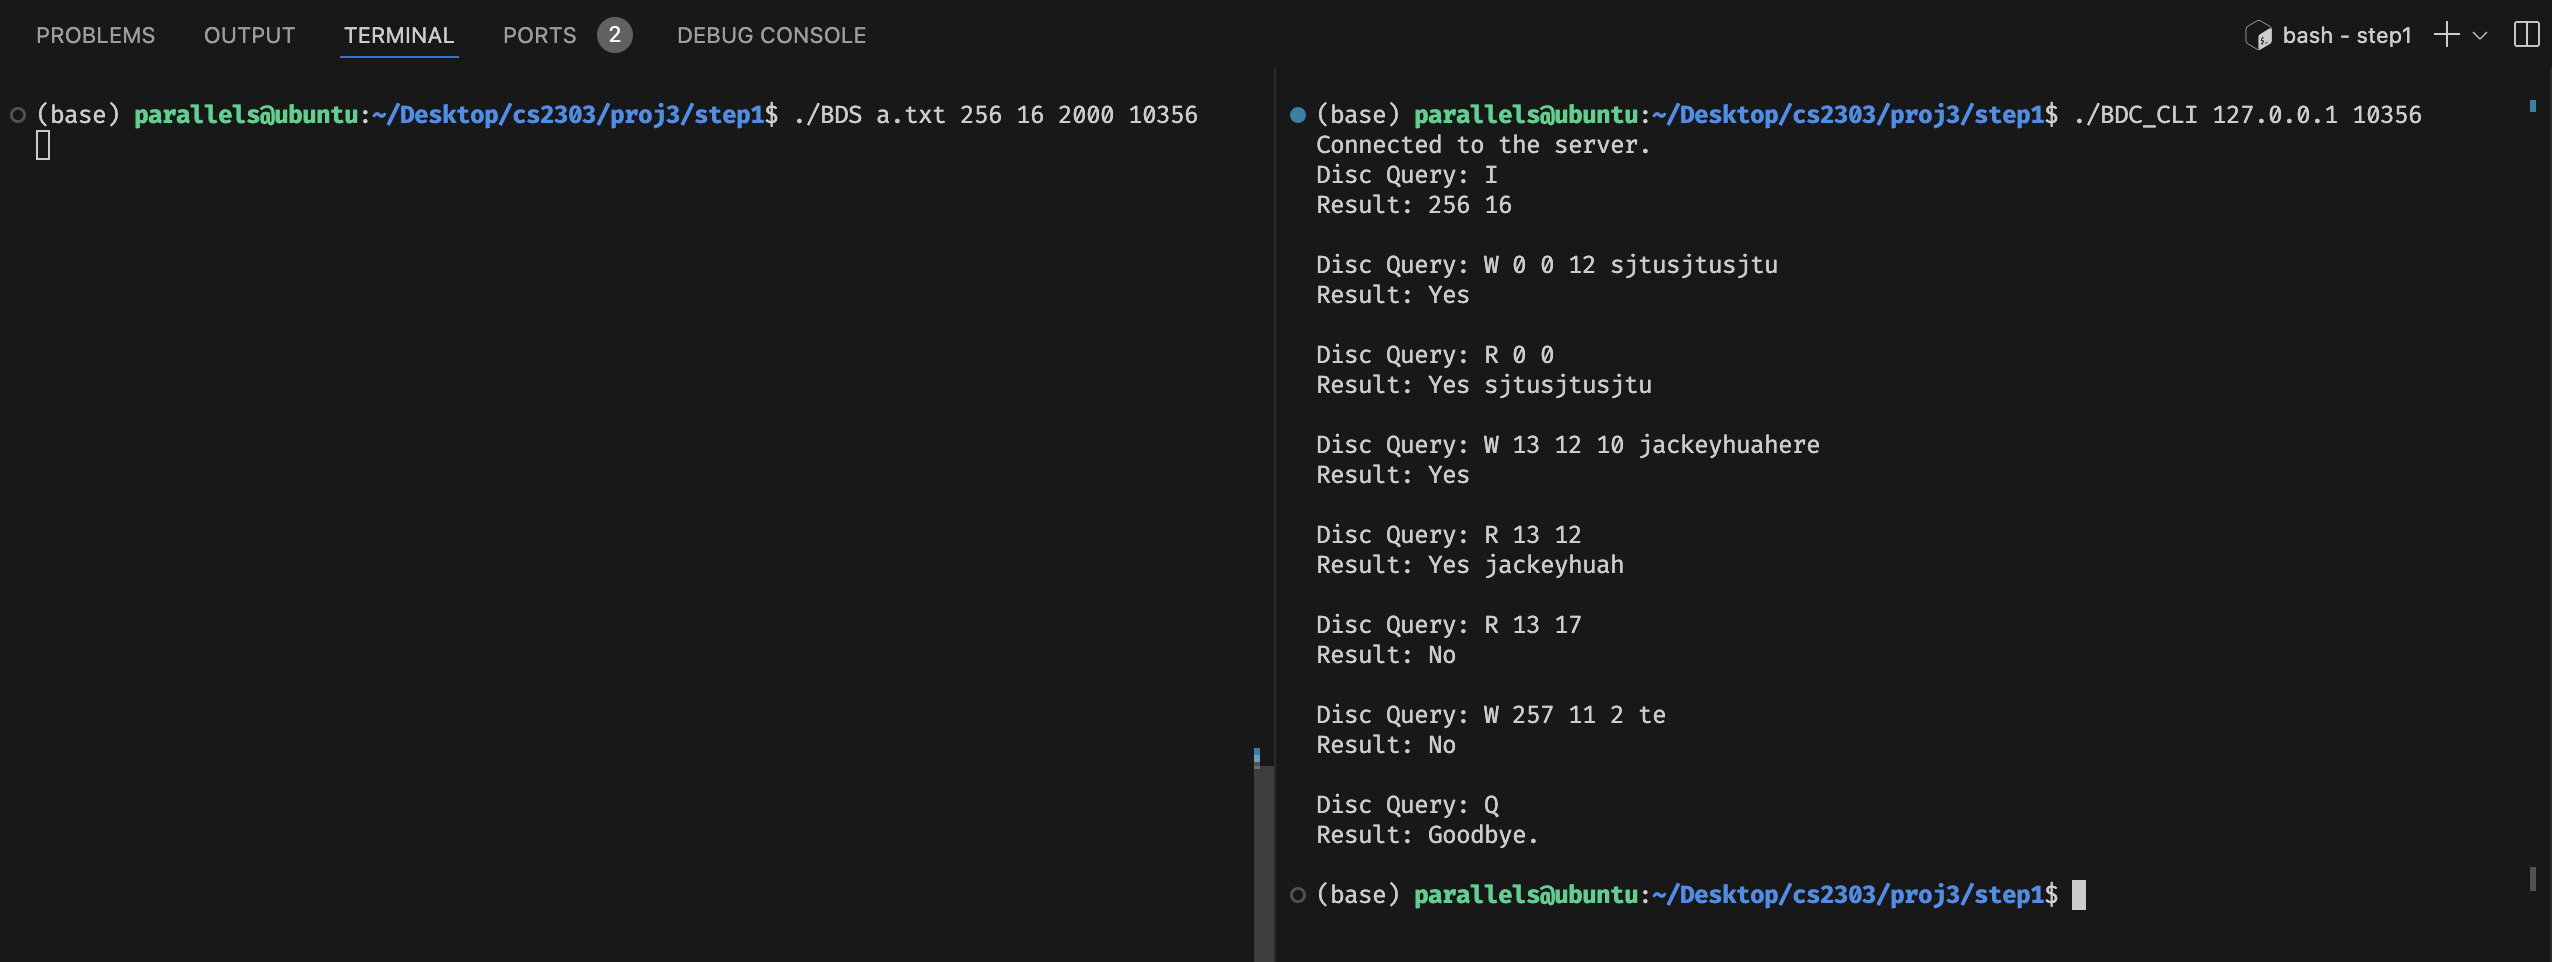
\includegraphics[width=0.8\textwidth]{fig/bdc_cli.png}
    \caption{Result of Command line input client.}
    \label{fig:cli}
\end{figure}

Then we run the BDC\_RANDOM with \texttt{./BDC\_RAND 127.0.0.1 10356 12}. 
Check Fig~\ref{fig:rnd} for the result. You can see that it generates 12 random read and write operations and prints out the result.
Note that as required, we do not print out the data that is read or written.

\begin{figure}[!h]
    \centering
    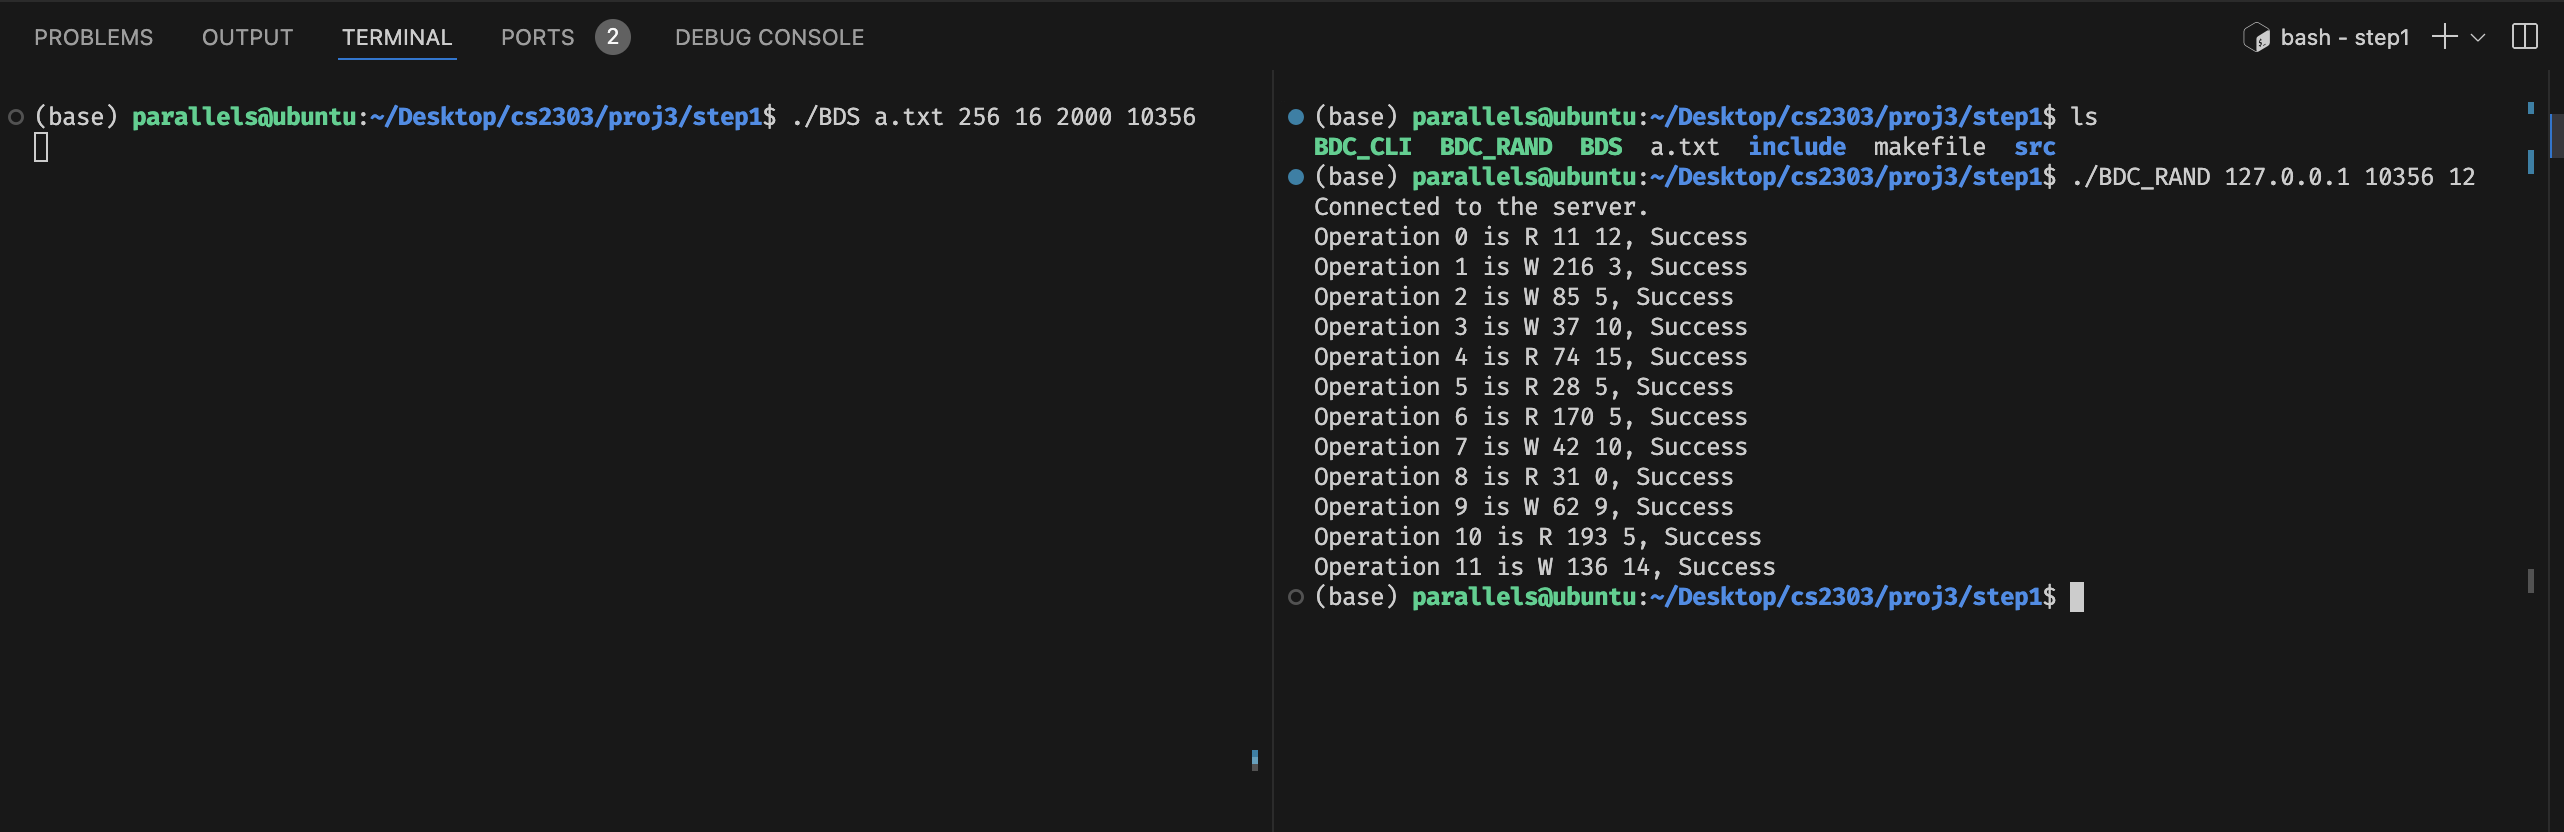
\includegraphics[width=0.8\textwidth]{fig/bdc_rnd.png}
    \caption{Result of Random input client.}
    \label{fig:rnd}
\end{figure}

\section{Step 2: Design a basic File System}
We copy \texttt{/step1} to \texttt{/step2/disc} and then modify the output of the disc.
It \textbf{no longer prints out Yes and No}, it just prints out the data. 

\textbf{Please do not use the old disc server. Instead, use the one in \texttt{proj3/step2/disc}}.

\subsection{Related Data Structure}
There are three new data structures in this step. They are \texttt{Entry, Inode, Superblock}. They are defined in \texttt{step2/include/\{name\}.h} and implemented in \texttt{step2/src/\{name\}.c}.
The design of these data structure are based on the slides and Linux file system.

Before we dive into the details of these data structures, we need to clarify how they are used in the file system.

Like Linux Ex2, the disc is separated into three parts, \textbf{superblock, inode and ordinary blocks}. Suppose that a block has size 256 bytes. Our 
superblock has size 652 bytes which needs 3 blocks to store. Our inode has size 32 bytes and we support 1024 inode, which needs 128 blocks to store.
So the reserve block for the meta data of the disc takes 131 blocks. The rest are all ordinary blocks. Check Fig~\ref{fig:layout} for the layout of the disc.

\begin{figure}[!h]
    \centering
    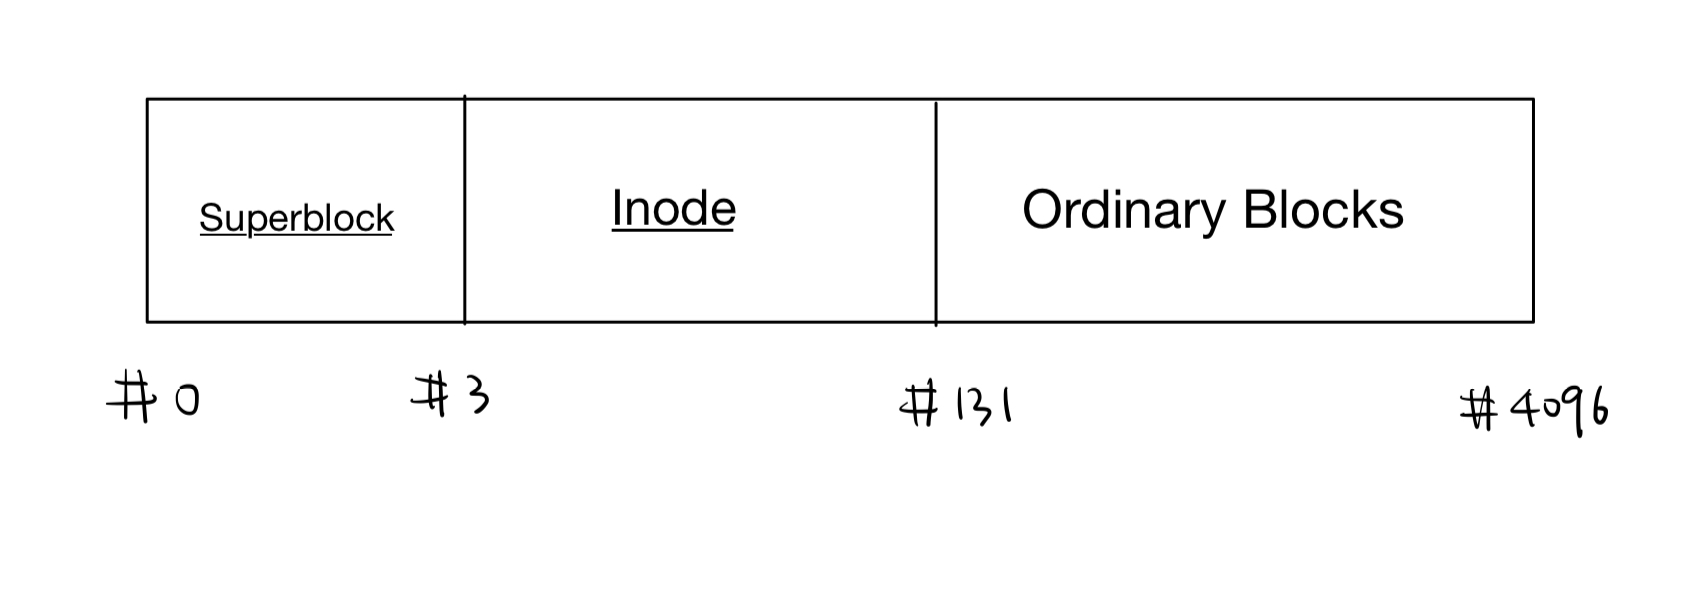
\includegraphics[width=0.8\textwidth]{fig/layout.jpeg}
    \caption{Memory layout of the disc.}
    \label{fig:layout}
\end{figure}

\texttt{Superblock} struct is used to manage thr superblock area of the disc, and \texttt{Inode} struct is used to manage the inode area of the disc, in which 8 inodes are grouped together and stored in a block in the disc.

In terms of the ordinary blocks, they are mainly used in 3 ways. First, they are used as the file content of file inode. All the information on this block is valid data of the file. Second, they are used as the block of the indirect block number of a \texttt{file type inode}.
All the data of this block is integers that represent indirect and valid block numbers of this file inode. Since a block is 256 bytes and a \texttt{uint16\_t} type integer is 2 bytes, so we can store 128 integers in this block. 
Third, they are treated as an entry if the inode is directory type. So \texttt{Entry} struct is used to manage the entry area of directory type inode.

\textbf{Note that, in directory type inode, we do not use indirect block area, since it is unnecessary and will bring additional developing burden.}

\textbf{Also note that, in the design of the following data structure, we use \texttt{uint\_t} type defined in \texttt{stdint.h} header file.}

\subsubsection{Wrapper design}
Given that we have frequent read/write operations into the disc, we should provide a unified interface to deal with the read/write operation. So comes \texttt{wrapper.h and wrapper.c}.
There are three main functions, \texttt{query, read1, and write1}.

\texttt{query} is simple, it sends \texttt{I} commands to the server and then receives the response from the server and stores the answer into a buffer. File server can visit the buffer and read the answer.

\texttt{read1} is used to read data at given index of the disc. It utilizes the syntax sugar of \texttt{readOp\_client()} function in \texttt{disc.c}. We send \texttt{R index} to the server and then receive the response from the server and stores the answer into a buffer.

\texttt{write1} is a little bit special. It should handle arbitrary long data, not just writing into A specific block. So we first calculate how many consecutive blocks we need to write the data into. Then we start a loop, in each iteration, we send part of the data to the server and write them into corresponding blocks. 

We suppose that the sockfd provided as parameters has been established, thus omitting the connection part.

The sketch of the code is as follows. I only shows the skeleton of \texttt{write1} function.

\begin{lstlisting}[language=C]
void write1(int sockfd, uint16_t client_id, int index, long size, void* data) {
    int rnd = (size + BLOCK_SIZE - 1) / BLOCK_SIZE;
    for (int i = 0; i < rnd; ++i) {
        // * Send W index len data to the server
        ...
    }
}
\end{lstlisting}

We can see a interesting parameter in the function, which is \texttt{client\_id}. I take multi-client requirements into account in this part,
 so that every client will be assigned a unique id. When the wrapper receives commands from a particular server, it will write the response 
 of the disc server to the corresponding index in the \texttt{extern char buffer[MAX_CLIENTS][MAX_LENGTH]} in \texttt{wrapper.h}.

\subsubsection{Superblock Data Structure}
We mimic the design of Linux superblock and takes the reference design from the slides into account.

In superblock, we need to trace how many inodes and blocks have been used, and how many of them are still vacant and available. We 
need to trace which index of the inodes and blocks are occupied and which are not. We also need to store the root inode id, which is the root directory of the whole file system.

Given the requirements stated above, i design the superblock struct as follows.

\begin{lstlisting}[language=C]
#define INODE_BITMAP_SIZE 32
#define BLOCK_BITMAP_SIZE 128
    // * We need 3 blocks to store the superblock
typedef struct {
    uint16_t _inode_count;
    uint16_t _block_count;
    uint16_t _vacant_inode_count;
    uint16_t _vacant_block_count;
    uint16_t _root_inode_id;
    uint32_t _inode_bitmap[INODE_BITMAP_SIZE];  // * 0 for vacant, from left to right
    uint32_t _block_bitmap[BLOCK_BITMAP_SIZE];
} Superblock;
\end{lstlisting}

The first 4 fields are used to store the count of used inodes, blocks, vacant inodes and blocks. 
The last 2 fields are bitmaps, which are worth noting. The basic element of the bitmap is a \texttt{uint32\_t} type integer.
Each bit has a unique id. The mechanism of the index is to count from left to right in the array, and in each element of the array, count from the 
MSB(Most significant bit) to the LSB(Least significant bit). Every binary bit of the interger is 0 or 1. If it is 0, it means that the inode/block of the corresponding index is vacant, otherwise, it is occupied.

Then we dive into related \textbf{opetation functions} of the superblock.

We first expand on \textbf{\texttt{update\_spbk()}}, it is a function that updates the superblock area to the disc, which is a necessary step if we have modified the superblock.
It copies the superblock into a buffer and writes it into disc via \texttt{write1()} provided by \texttt{wrapper.h}. The code is as follows.

\begin{lstlisting}[language=C]
void update_spbk() {
    char data[BLOCK_SIZE * 3 + 10];
    memcpy(data, &spbk, sizeof(Superblock));
    write1(sockfd, 0, 0, sizeof(Superblock), data);
}

\end{lstlisting}

Then we talk about how to initialize the superblock variable \texttt{spbk} in \texttt{superblock.c} via \textbf{\texttt{init\_spbk()}}. It is a function that initializes the superblock area of the disc.
We first check the block size of real disc, if it is too large, it will be truncated into 4096.
If it is too small, even smaller than reserve block numbers, we will exit with error message.
We do not have used inode at the beginning, while we have used 131 reserved blocks for superblock and 1024 inodes. We set the root inode id to be 0.
Since we don't use any inodes, the bitmap of inodes are all 0. Since we have used 131 blocks, 
we need to set the first 3 elements in block bitmap to be \texttt{UINT32_MAX or -1}, and the top 3 bits of the 4th element to be 1.
Notice that we have a static variable called \texttt{sockfd} in this source file, it is used to appoint the file descriptor of read/write operation. We need to 
provide this file descriptor in the parameters and then assign it to \texttt{sockfd}. After that, we can write the superblock to the disc via \texttt{update\_spbk()}.

\begin{lstlisting}[language=C]
    static int sockfd;
    Superblock spbk;
    
    void init_spbk(int block_size, int fd) {
        // block size check 
        ... 
        spbk._inode_count = 0;
        spbk._block_count = RESERVE_BLOCK_NUM;
        spbk._vacant_inode_count = MAX_INODE_NUM;
        spbk._vacant_block_count = real_block_size - RESERVE_BLOCK_NUM;
        spbk._root_inode_id = 0;
        memset(spbk._inode_bitmap, 0, sizeof(spbk._inode_bitmap));
        memset(spbk._block_bitmap, 0, sizeof(spbk._block_bitmap));
        for (int i = 0; i <= 3; ++i) {
            spbk._block_bitmap[i] = -1;
        }
        uint32_t mask = (1 << 31) | (1 << 30) | (1 << 29);
        spbk._block_bitmap[4] |= mask;
        sockfd = fd;
        update_spbk();
    }    
\end{lstlisting}

Then we talk about how to allocate a new block via \textbf{\texttt{alloc\_block()}}. It is a function that allocates a new block for the file system.
We check the block bitmap from left to right in order, and check whether there is a bit that is 0. If found, we set it to 1, update \texttt{block\_count} and \texttt{vacant\_block\_count} in the superblock, and return the index of the block.
If all the bits are 1, we return -1 to indicate that there is no vacant block. The code is as follows.

\begin{lstlisting}[language=C]
int alloc_block() {
    ... 
    int blockID = -1;
    for (int i = 4; i < BLOCK_BITMAP_SIZE; ++i) {
        for (int j = 31; j >= 0; --j) {
            if ((spbk._block_bitmap[i] >> j) & 1) continue;
            else {
                blockID = i * 32 + 32 - j;
                spbk._block_bitmap[i] |= (1 << j);
                spbk._block_count++;
                spbk._vacant_block_count--;
                // update block omits
                ... 
                return blockID;
            }
        }
    }
    // * Do not find vacant block
    return blockID;
}
\end{lstlisting}

Finally, we talk about how to free a block via \textbf{\texttt{gc\_block()}}. It is the abbreviation of garbage collection block. It is a function that frees a block for the file system.
We do not allow to free reserve blocks or invalid index blocks. If met, we return -1 to indicate that the operation is invalid.
Then we need to find in which index are the current block in the bitmap array. It is easy to verify that it is in the \texttt{blockID / 32} index of the array, and the bit index is \texttt{blockID \% 32}.
Then we set the corresponding bit from 1 to 0, and update the \texttt{block\_count} and \texttt{vacant\_block\_count} in the superblock. 
Then we manually write 0 length data into the blockID via \texttt{write1()} so that it will be reformatted and set empty. At last, we update the superblock into the disc. The code is as follows.

\begin{lstlisting}[language=C]
    int gc_block(uint16_t blockID, uint16_t clientID) {
        // check whether blockID is valid Omits
        ... 
        int c = blockID / 32;
        int r = blockID % 32;
        if (((spbk._block_bitmap[c] >> (31 - r)) & 1) == 0) {
            return 1;
        }
        spbk._block_count--;
        spbk._vacant_block_count++;
        spbk._block_bitmap[c] ^= (1 << (31 - r));
        write1(sockfd, clientID, blockID, 0, "");
        update_spbk();
        return 1;
    }       
\end{lstlisting}

\subsubsection{Entry Data Structure}
As is described in the previous section, the entry struct is used to manage the entry area of directory type inode. 
In the linux file system, entry mainly focus on the name of the file and the inode number of the file. So in my design, 
i track the inode id, name, type and state of the file/directory that this entry represents.
In terms of type, if the value is 0, then it is a file. If the value is 1, then it is a directory. In terms of state, if the value is 0, then it is vacant. If the value is 1, then it is occupied.
The inode id is important when we want to access the file/directory because their detailed information is stored in the inode area of the disc.
The name field is the only space that will keep track of the name of the file/directory. We do not store it in inode as Linux does.

The struct is as follows. There are no special operations for this struct, so we omit the operation functions.

In order to align, we specially set the length of the name to be 28, so that the size of the struct is 32, which can divide 256 evenly. Namely, we can store exactly
8 entries in a block.

\begin{lstlisting}[language=C]
#define MAX_NAME_LEN 28
typedef struct {
        uint8_t _type;
        uint8_t _state;
        uint16_t _inode_id;
        char _name[MAX_NAME_LEN];
    } Entry;
        
\end{lstlisting}

\subsubsection{Inode Data Structure}
This is the most important part of the file system. Inode is used to manage the inode area of the disc which keeps track of meta data of the current node.
Like Linux and slides, we need to keep track of the type, link number, file size, last modified time, inode index, parent index, direct block, indirect block. For the 
sake of part 3, i add permission and owner id also into the struct. 

\textbf{Type} maintains whether the inode represents a file or a directory, 0 for the former and 1 for the latter.
\textbf{Link number} maintains how many blocks are related to this inode, namely the count of valid blocks in the direct block and indirect block.
\textbf{File size} is valid only for file type inode, and maintains the size of the file.
\textbf{Last modified time} is the time when the inode is last modified.
\textbf{Inode index} is the index of current inode, and \textbf{parent index} is the index of the parent inode, which is crucial when we meet \texttt{cd ..} commands. Given that some inodes like the root
may not have root, let's suppose \texttt{UINT16_MAX or 65535} to be the sign of not exist.
\textbf{Direct block} is an array that maintains the index of the direct block that the inode points to. If the inode is a file, it is used to store the contents. If 
the inode is a directory, it is used to store the entry. 
\textbf{Indirect block} is only valid when this is a file inode. It is used to store the index of the indirect block that the inode points to. In the indirect block, we can see at most
128 integers, which represent the index of the block that the file inode indirectly points to. 
\textbf{Permission} stores the read/write/execute permission of owner and other users. We always suppose the root is the super user, and can do anything. Check Fig~\ref{fig:permission} for the permission design.
\textbf{Owner id} stores the owner id of the file/directory. It is key to part 3. Because we need to check whether the current user is owner and has the necessary permission to access the file/directory.

\begin{figure}[!h]
    \centering
    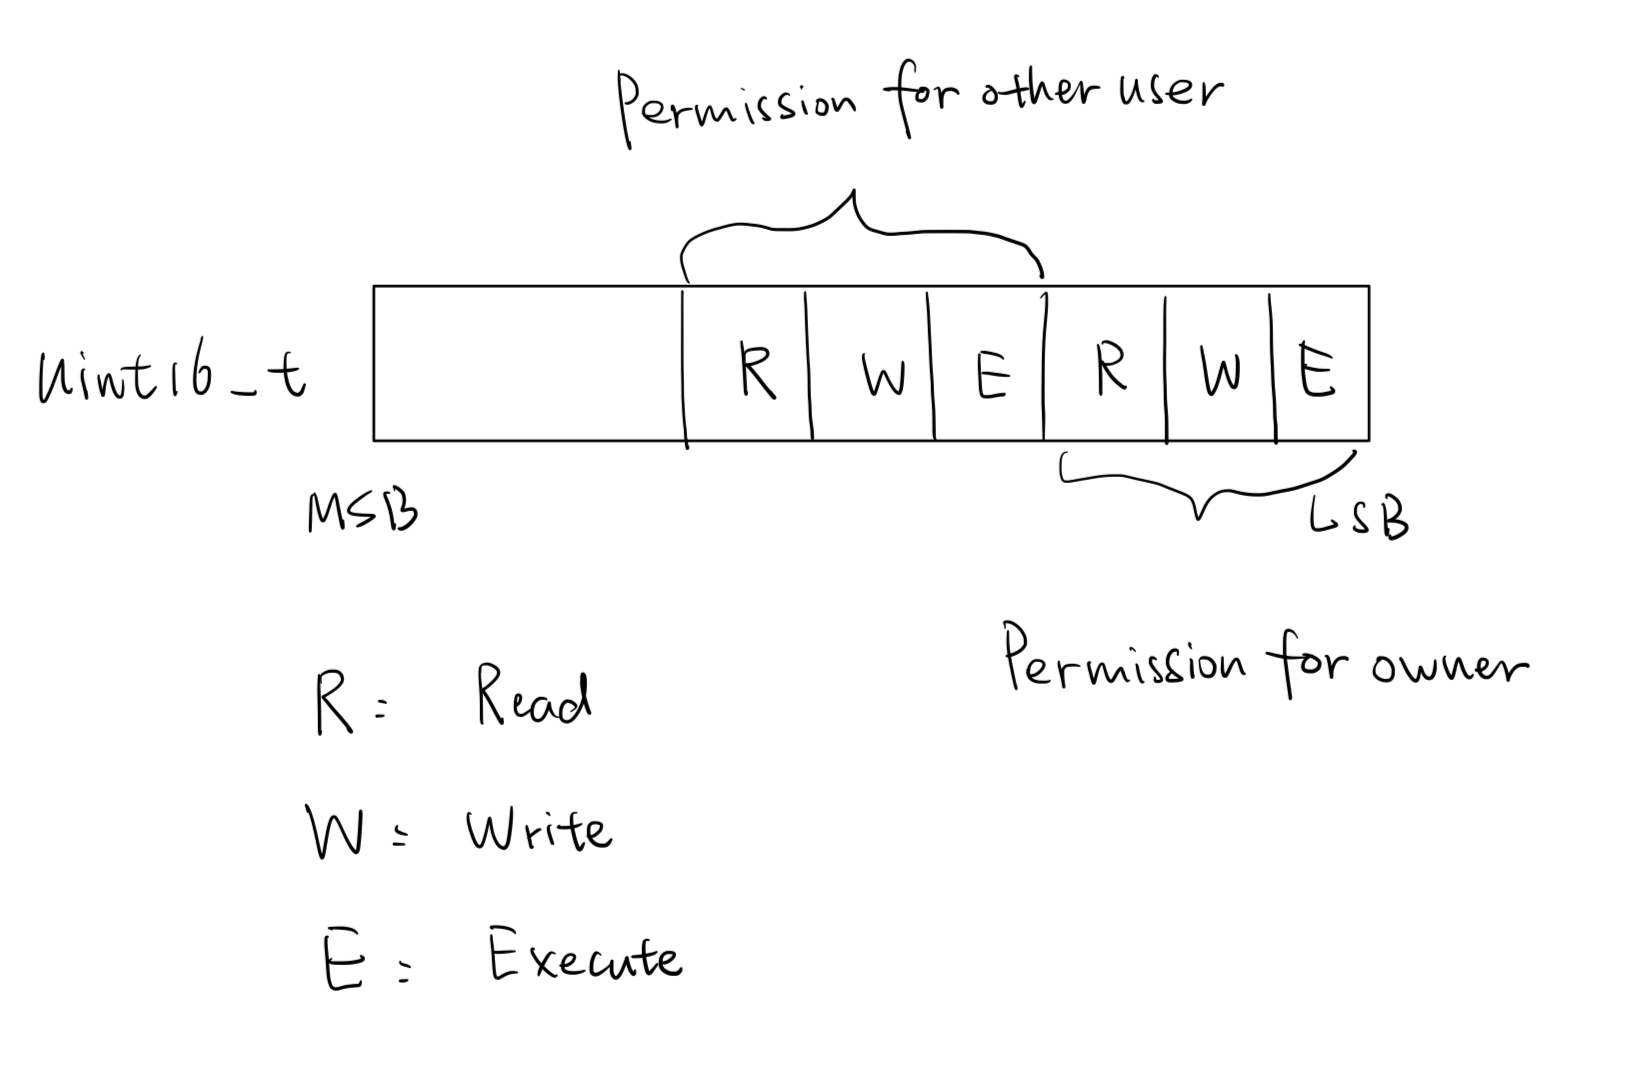
\includegraphics[width=0.8\textwidth]{fig/permission.jpeg}
    \caption{Permission design.}
    \label{fig:permission}
\end{figure}

It is worth noting that i fully utilize word alignment in C and adjust the size of direct block array to be 7, so that the size of the struct is 32, which can divide 256 evenly. Namely, we can store exactly
8 inodes in a block.

The struct is as follows. 

\begin{lstlisting}[language=C]
    #define DIRECT_LINK 7

    typedef struct {
        uint8_t _mode;                           // * 0 for file and 1 for dir
        uint8_t _direct_count;                   // * # of links associated with this file
        uint16_t _file_size;                     // * file size
        uint32_t _last_modified_timestamp;       // * timestamp
        uint16_t _index;                         // * current inode index
        uint16_t _fa_index;                      // * father inode index, -1 for not exist (65535)
        uint16_t _direct_block[DIRECT_LINK];     // * direct block link, store block id
        uint16_t _indirect_block;                // * indirect block link, one level
        uint16_t _permission;                    // * only low 6 bits are valid, owner & group permission
        uint16_t _ownerID;                       // * owner ID
    } Inode;
    
    extern Inode inode_table[MAX_INODE_NUM];
\end{lstlisting}

Then we focus on the operation functions of the inode struct. I divide these functions into 4 type,
\textbf{initialization, inode level, file level, and directory level}.

We first look at the \textbf{initialization function \texttt{void init\_root(int)}}. The root exists as soon as we format the disc, so 
i design a special function for it. The root is a directory and does not have any link count.
The index for it is set to 0, and since it does not have parent, its parent index is set to 65535.
Its owner ID is root, and we suppose that root is always 0. The permission is set to 63, which means that the owner can read/write/execute, and the group and other users can read/write/execute.
In reality, i set the permission to be -1, namely \texttt{UINT16_MAX}, which is just a fast way to do that. 
Apart from that, we need to modify the inode bitmap in superblock to indicate that the root inode (at index 0) is occupied.
Like the design in \texttt{superblock.c}, we add a static variable \texttt{sockfd} to store the file descriptor of read/write operation. And we
 need to provide this file descriptor in the parameters and then assign it to \texttt{sockfd}. 

So the code for this function is as follows.

\begin{lstlisting}[language=C]
void init_root(int fd) {
    Inode root;
    memset(inode_table, 0, sizeof(inode_table));
    inode_table[0]._mode = 1;
    inode_table[0]._direct_count = 0;
    inode_table[0]._last_modified_timestamp = time(NULL);
    inode_table[0]._file_size = 0;
    inode_table[0]._index = 0;
    inode_table[0]._fa_index = 65535;
    memset(inode_table[0]._direct_block, 0, sizeof(inode_table[0]._direct_block));
    inode_table[0]._indirect_block = 0;
    inode_table[0]._permission = -1;
    inode_table[0]._ownerID = 0;
    spbk._inode_bitmap[0] |= (1 << 31);
    sockfd = fd;
    update_spbk();
}
\end{lstlisting}

Another initialization function is \textbf{\texttt{update_inode_table()}}. Like \texttt{update\_spbk()}, it  
justs writes the whole inode table back to the disc. I omit the code here.

Then we talk about the \textbf{inode level operation functions}. We first look at the \textbf{\texttt{alloc\_inode()}} function. It is a function that allocates a new inode for the file system.
Like the \texttt{alloc\_block()} function, we check the inode bitmap from left to right in order, check from MSB to LSB in order, and check whether there is a bit that is 0. If found, we set it to 1, update \texttt{inode\_count} and \texttt{vacant\_inode\_count} in the superblock, and return the index of the inode.
If all the bits are 1, we return -1 to indicate that there is no vacant inode. The code is as follows.

\begin{lstlisting}[language=C]
    int alloc_inode() {
        ...
        int inodeID = -1;
        for (int i = 0; i < INODE_BITMAP_SIZE; ++i) {
            for (int j = 31; j >= 0; --j) {
                if ((spbk._inode_bitmap[i] >> j) & 1) continue;
                else {
                    inodeID = i * 32 + 32 - j;
                    spbk._inode_bitmap[i] |= (1 << j);
                    spbk._inode_count++;
                    spbk._vacant_inode_count--;
                    update_spbk();
                    return inodeID;
                }
            }
        }
        return inodeID;
    }    
\end{lstlisting}

After that, we talk about \textbf{\texttt{gc_inode()}} which is aimed to free all the block resources in current inode. \textbf{We 
do not need to recursive free the resouces in possible subdirectory, we have special function for that purpose.}
We do not allow to free the root node, so i add a special check at the beginning. 
We then check the elements in direct block array, if it is not 0, we free the block via \texttt{gc\_block()}.
After that, we check the indirect block, if it is not 0, we first load the indirect block and assign it to a \texttt{uint16_t[128]} type 
array. Then we free all the blocks in the array via \texttt{gc\_block()}. At last, we free the indirect block itself.
Finally, we modify the inode bitmap in superblock to indicate that the current inode is vacant. The code is as follows.

\begin{lstlisting}[language=C]
int gc_inode(Inode* inode, uint16_t clientID) {
    ... 
    for (int i = 0; i < DIRECT_LINK; ++i) {
        gc_block(inode->_direct_block[i], clientID);
    }

    if (inode->_indirect_block != 0) {
        // * Have an indirect block
        read1(sockfd, clientID, inode->_indirect_block);
        uint16_t indirect_blockid[128];
        memcpy(indirect_blockid, buffer[clientID], BLOCK_SIZE);
        for (int i = 0; i < 128; ++i) {
            gc_block(indirect_blockid[i], clientID);
        }
        gc_block(inode->_indirect_block, clientID);        
    }

    spbk._inode_bitmap[c] ^= (1 << (31 - r));
    spbk._inode_count--;
    spbk._vacant_inode_count++;
    update_spbk();
    return 0;
}
\end{lstlisting}

Then, we look at how to recursively free a directory inode via \textbf{\texttt{gc_inode_recursive()}}. Since
 a directory inode does not use the indirect block, so we only need to look at direct block array. 
Since the direct block stores 8 entry, so we first load the block and assign it to a \texttt{Entry[8]} type array. 
Then we check whether the entry is valid, if yes, we check whether it is a file or a directory. If it is a file, we free the inode via \texttt{gc\_inode()}.
Otherwise, we recursively call \texttt{gc\_inode\_recursive()} to free the directory inode. At last, we free the block itself and then modify the inode bitmap as stated in the \texttt{gc\_inode()} part. The code is as follows.

\begin{lstlisting}[language=C]
    int gc_inode_recursive(Inode* inode, uint16_t clientID) {
        ... 
        Entry entry[BLOCK_SIZE / sizeof(Entry)];
        for (int i = 0; i < DIRECT_LINK; ++i) {
            if (inode->_direct_block[i] == 0) continue;
            read1(sockfd, clientID, inode->_direct_block[i]);
            memset(entry, 0, sizeof(entry));
            memcpy(entry, buffer[clientID], BLOCK_SIZE);
            for (int j = 0; j < BLOCK_SIZE / sizeof(Entry); ++j) {
                if (entry[j]._state == 0) {
                    continue;
                } else {
                    if (entry[j]._type == 1) {
                        gc_inode_recursive(&inode_table[entry[j]._inode_id], clientID);
                    } else {
                        gc_inode(&inode_table[entry[j]._inode_id], clientID);
                    }
                }
            }
            gc_block(inode->_direct_block[i], clientID);
        }
        ... 
        // Same as gc_inode
    }
        
\end{lstlisting}

I also provide a \texttt{write_inode_to_disc()} to write a specific inode back to the disc, and a \texttt{init_inode()}
 function to init a given inode with given parameters. They are trivial and i omit the code here.


After that we focus on the \textbf{dir level operation functions}. We first look at the \textbf{\texttt{dir_check_existence}} function. 
It checks whether there is a file/directory in current inode that has the same name and type as the given name and type. We also need to make 
sure the current inode is a directory and load the direct block of the current inode. Then we traverse through every entry to have a check. If found, we return the inode id of the file/directory. If not found, we return -1. 
We still omit the code here, since it is trivial.

Then we talk about the \textbf{\texttt{dir_add_entry}} function. It is a function that adds a new entry to the current directory inode. We first check whether the current inode is a directory, and whether the entry already exists. If it exists, we return -1 to indicate that the operation is invalid. 
Then we check whether there is a vacant entry in the direct block. If found, we add the entry to the vacant entry and return 0 to indicate that the operation is successful. If not found, we return -1 to indicate that the operation is invalid. The code is as follows.

Then we talk about the \texttt{dir_add_entry()} function. It adds an entry of given name and type to the current directory inode.
So we first check whether the current inode is a directory. Then we check the already allocated direct block of the current inode. If there is a vacant entry in the direct block, we add the entry to the vacant entry and return 0 to indicate that the operation is successful. 
If there is no vacant entry, we do another traverse to check whether there is a vacant direct block. If found, we first allocate a block for this vacant direct block, and then add the entry to it, and return 0 to indicate that the operation is successful. If not found, we return -1 to indicate that the operation is invalid. The code is as follows.
Before we do the traverse, we can do a simple check to see whether the entry already exists via \texttt{dir\_check\_existence()}. If found, just return 0, otherwise proceed to the next step. 
The code is as follows.

\begin{lstlisting}[language=C]
    int dir_add_entry(Inode* inode, uint16_t clientID, char* name, uint8_t mode) {
        // * Make sure it is a DIR type inode
        if (inode->_mode != 1) {
            return -1;
        }
        if (dir_check_existence(inode, mode, name) != -1) return 0;
        Entry entry[BLOCK_SIZE / sizeof(Entry)];
        char wb_buf[BLOCK_SIZE];
        // * We first check if there are vacant entry in allocated block
        int i = 0;
        for (; i < DIRECT_LINK; ++i) {
            if (inode->_direct_block[i] == 0) continue;
            read1(sockfd, clientID, inode->_direct_block[i]);
            memset(entry, 0, sizeof(entry));
            memcpy(entry, buffer[clientID], BLOCK_SIZE);
            for (int j = 0; j < BLOCK_SIZE / sizeof(Entry); ++j) {
                if (entry[j]._state == 1) continue;
                // find a vacant entry and do the initialization
                ... 
                return 1;
            }
        }
        // * No vacant entry in allocated block
        // * Try allocate new vacant block
        i = 0;
        for (; i < DIRECT_LINK; ++i) {
            if (inode->_direct_block[i] != 0) continue;
            // find a vacant block and do the initialization
            ... 
            return 1;
        }
        return -1;
    }    
\end{lstlisting}

Then we look at \texttt{dir_del_entry()}. It is a function that deletes an file entry of given name from the current directory inode.
We first check whether the current inode is a directory. Then we check whether the entry exists via \texttt{dir\_check\_existence()}. If not found, we return -1 to indicate that the operation is invalid.
Otherwise, we traverse through all valid direct blocks, load it into a \texttt{Entry[8]} type array, and then check whether the entry exists in the array. If found, we set the state of the entry to 0 to indicate that it is vacant, and \texttt{gc\_inode()} to free the target inode.
At last, we need to modify the time stamp of the current inode and update current inode into the disc. The code is as follows.

\begin{lstlisting}[language=C]
    int dir_del_entry(Inode* inode, uint16_t clientID, char* name) {
        if (inode->_mode != 1) return -1;
        int id = dir_check_existence(inode, 0, name);
        if (id == -1) return 0;
        Entry entry[BLOCK_SIZE / sizeof(Entry)];
        char wb_buf[BLOCK_SIZE];
        for (int i = 0; i < DIRECT_LINK; ++i) {
            if (inode->_direct_block[i] == 0) continue;
            // load the block into entry array
            ... 
            for (int j = 0; j < BLOCK_SIZE / sizeof(Entry); ++j) {
                if (entry[j]._state == 0) continue;
                if (strcmp(entry[j]._name, name) == 0 && entry[j]._type == 0) {
                    // find the target 
                    ...
                    entry[j]._state = 0;
                    gc_inode(&inode_table[id], clientID);
                    inode->_last_modified_timestamp = time(NULL);
                    write_inode_to_disc(inode, clientID, inode->_index);
                    return 1;
                }
            }
        }
    }    
\end{lstlisting}

Then we look at \texttt{dir_del_entry_recursive()}, it is a function that recursively deletes a directory inode and all its subdirectory and files, which is pretty like \texttt{rm -r} command in Linux.
It is pretty like \texttt{dir_del_entry()}. It just replaces the \texttt{gc_inode()} with \texttt{gc_inode_recursive()}. And the if condition needs to make sure the entry type is a directory. The code is as follows.

\begin{lstlisting}[language=C]
    ...
    if (strcmp(entry[j]._name, name) == 0 && entry[j]._type == 1) {
        ...
        entry[j]._state = 0;
        gc_inode_recursive(&inode_table[id], clientID);
        inode->_last_modified_timestamp = time(NULL);
        write_inode_to_disc(inode, clientID, inode->_index);
        return 1;
    }    
    ... 
\end{lstlisting}

After that, we should take a look at \texttt{dir_ls()}, it is a function that lists all the files and directories in the current directory inode.
It first checks whether the current inode is a directory type inode, then load and traverse through every valid direct block. If the entry is valid, it will
concatenate the name into a buffer. After the traverse, it will copy the buffer to the answer pointer which is provided as a parameter.
Specifically, in order to distinguish between file and directory, i add \textbf{green color} for directory name.
The code is as follows.

\begin{lstlisting}[language=C]
    void dir_ls(Inode* inode, char* ans) {
        if (inode->_mode == 0) return;
        Entry entry[BLOCK_SIZE / sizeof(Entry)];
        for (int i = 0; i < DIRECT_LINK; ++i) {
            if (inode->_direct_block[i] == 0) continue;
            // load the block into entry array
            ...
            for (int j = 0; j < BLOCK_SIZE / sizeof(Entry); ++j) {
                if (entry[j]._state == 0) continue;
                if (entry[j]._type == 1) {
                    // green color for directory
                    strcat(buf, "\033[1;32m");
                    strcat(buf, entry[j]._name);
                    strcat(buf, "\033[0m ");
                } else {
                    strcat(buf, entry[j]._name);
                    strcat(buf, " ");
                }
            }
        }
        strcpy(ans, buf);
    }        
\end{lstlisting}

Finally, we step into \textbf{\texttt{file level operation functions}}. We first look at \texttt{file\_read()}. It writes all the contents of the current file inode
into a answer pointer provided as a parameter. We check whether the current inode is a file type inode, then check whether the link count is less or equal than the size of direct block.
If it is, we just need to load \texttt{inode->_direct_count} direct blocks and concatenate their contents into a buffer. If not, 
we need to load all the direct blocks and concatenate their contents into a buffer, and then load the indirect block and load the first \texttt{inode->_direct_count - DIRECT\_LINK} blocks and concatenate the contents into the buffer. The code is as follows.

\begin{lstlisting}[language=C]
    
void file_read(Inode* inode, uint16_t clientID, char* ans) {
    if (inode->_mode == 1) return;
    char buf[BLOCK_SIZE + 1];
    int last_block_size = inode->_file_size % BLOCK_SIZE;

    if (inode->_direct_count <= DIRECT_LINK) {
        for (int i = 0; i < inode->_direct_count; ++i) {
            if (inode->_direct_block[i] == 0) return;   // * Error
            // load the block 
            ... 
            strcat(ans + i * BLOCK_SIZE, buf);
        }
    } else {
        for (int i = 0; i < DIRECT_LINK; ++i) {
            if (inode->_direct_block[i] == 0) return;   // * Error
            // load the block
            ... 
            strcat(ans + i * BLOCK_SIZE, buf);
        }
        if (inode->_indirect_block == 0) return;   // * Error
        read1(sockfd, clientID, inode->_indirect_block);
        uint16_t indirect_blockid[128];
        memcpy(indirect_blockid, buffer[clientID], BLOCK_SIZE);
        for (int i = 0; i < inode->_direct_count - DIRECT_LINK; ++i) {
            // load the block 
            ... 
            strcat(ans + (i + DIRECT_LINK) * BLOCK_SIZE, buf);
        }
    }
}

\end{lstlisting}

At last, we look at \texttt{file\_write()}. It writes the given data into the current file inode. 
We need to enumerate the cases. I first check whether the block necessary to store the data is smaller or equal to \texttt{inode->direct\_count}. If it is, we then check whether the necessary block number is smaller or equal to \texttt{DIRECT\_LINK}. 
If it is, we just need to write the data into direct blocks and clear the rest of direct blocks and possible indirect block. Otherwise, 
we first need to write data to all direct blocks, and then write the rest of the data to the indirect block, then clear the rest of indirect blocks.
If the block necessary to store the data is larger than \texttt{inode->direct\_count}, we still check whether the necessary block number is smaller or equal to \texttt{DIRECT\_LINK}.
If it is, we first need to write data to all allocated direct blocks, and allocate new block as needed, then write data into newly allocated blocks.
If it is not, we first need to write data to all allocated direct blocks, and allocate new block as needed, then write data into newly allocated blocks, and allocate new indirect block as needed, then write data into newly allocated indirect blocks. The code is as follows.
Since the code is too long, i just present the major if-else structure and omit the details.

\begin{lstlisting}[language=C]
    void file_write(Inode* inode, uint16_t clientID, char* src) {
        if (inode->_mode == 1) return;
        int need = (strlen(src) + BLOCK_SIZE - 1) / BLOCK_SIZE; // * ceil(strlen(src) / BLOCK_SIZE)

        if (need <= inode->_direct_count) {
            if (need <= DIRECT_LINK) {
                for (int i = 0; i < need; ++i) {
                    if (inode->_direct_block[i] == 0) return; // ! Never happen
                    // write data to the block
                    ...
                }
                // free the rest of direct blocks and possible indirect block
                ...
            } else {
                for (int i = 0; i < DIRECT_LINK; ++i) {
                    if (inode->_direct_block[i] == 0) return; // ! Never happen
                    // write data to the block
                    ...
                }
                if (inode->_indirect_block == 0) return;  // ! Never happen
                uint16_t indirect_blockid[128];
                // load indirect block
                ...
                for (int i = 0; i < need - DIRECT_LINK; ++i) {
                    if (indirect_blockid[i] == 0) return; // ! Never happen
                    // write to indirect block
                    ...
                }
                // free the rest of indirect blocks
                ...
            }
        } else {
            if (need <= DIRECT_LINK) {
                for (int i = 0; i < need; ++i) {
                    // write data and allocate block as needed
                    ...
                }
            } else {
                for (int i = 0; i < DIRECT_LINK; ++i) {
                    // write data and allocate block as needed
                    ...
                }
                uint16_t indirect_blockid[128];
                // load indirect block or allocate a new one
                
                for (int i = 0; i < need - DIRECT_LINK; ++i) {
                    // write to indirect block and allocate block as needed
                    ...
                }
            }
        }
    }    
\end{lstlisting}

\subsection{FS Design}
In this subsection, i will explain how to parse the command line input and the whole process of receiving a command line input and get the result.

\subsubsection{Command Line Input}
The structure i design is pretty like the disc server, which is in \texttt{parseCmd} function.
It uses \texttt{strtok} to split the command line input into several parts, and then check the first part to see which command it is.
Then it will call the corresponding function to handle the command. We support all the required commands in the project description, including \texttt{f, ls, cd, mkdir, mk, rm, rmdir, cat, w, r, i, d}.
Apart from that, we additionally support \texttt{e} command to exit. Since the code is too long, i only show a small snippet.

\begin{lstlisting}[language=C]
    void parseCmd(char* command) {
        char* token = strtok(command, " \n\r");
        char** argv = malloc(MAX_ARG * sizeof(char*));
        int i = 0;
        while (token != NULL) {
            argv[i++] = token;
            token = strtok(NULL, " \n\r");
        }
        argv[i] = NULL;
        if (i == 1) {
            if (strcmp(argv[0], "f") == 0) {
                fOp();
            } else if (strcmp(argv[0], "ls") == 0) {
                lsOp();
            } else if (strcmp(argv[0], "e") == 0) {
                eOp();
            } else {
                perror("Invalid command.");
            }
        } 
    }    
\end{lstlisting}

Most of the commands can directly use the corresponding functions provided by \texttt{inode.c}.
For example, 
\begin{itemize}
    \item \texttt{ls} command can directly call \texttt{dir\_ls()} to list all the files and directories in the current directory inode.
    \item \texttt{f} command can directly call \texttt{init\_spbk(), init\_root(), init\_inode()} to format and initialize the file system.
    \item \texttt{mk} command can directly call \texttt{dir\_add\_entry()} to add a new file entry to the current directory inode.
    \item \texttt{mkdir} command can directly call \texttt{dir\_add\_entry()} to add a new directory entry to the current directory inode.
    \item \texttt{rm} command can directly call \texttt{dir\_del\_entry()} to delete a file entry from the current directory inode.
    \item \texttt{rmdir} command can directly call \texttt{dir\_del\_entry\_recursive()} to delete a directory entry from the current directory inode.
    \item \texttt{cat} command can directly call \texttt{file\_read()} to read the contents of the current file inode.
    \item \texttt{w} command can directly call \texttt{file\_write()} to write the given data into the current file inode.
\end{itemize}

There are only 3 commands that need to be handled specially, which are \texttt{cd, i, d}.
Let's dive into these 3 commands.

First, we talk about \texttt{cd} command. It is a command that changes the current directory inode to the target directory inode. We suppose that the path provided as parameter is \textbf{RELATIVE PATH}.
We first need to parse the path into tokens separated by \texttt{/ or [backslash]n[backslash]r}. Before we proceed, we need to back up current path and inode id, in case something wrong
happens. Then we start to deal with every token from left to right. If the current token is \texttt{.}, we just skip, because it means the current directory. 
If the current token is \texttt{..}, we need to change to the parent directory. If this current inode has a parent inode, we change the current inode to the parent inode. And we need to modify the current path, removing the suffix until we meet the first \texttt{/}. But 
there is a special case, that the parent inode is root. If we remove the suffix as described, the path name array will be empty, so we need to add a \texttt{/} to the path name array. If 
the current token is neither \texttt{.} nor \texttt{..}, we need to check whether that entry exists in the current directory inode. If it exists, we change the current inode to the target inode. If not, we restore the current path and inode id, and return an error message. The code snippet is as follows.

\begin{lstlisting}[language=C]
void cdOp(char* name) {
    uint16_t backup = cur_inode_id;
    char* token = strtok(name, "/\n\r");
    char backup_path[MAX_BUFFER_LENGTH];
    memset(backup_path, 0, MAX_BUFFER_LENGTH);
    strcpy(backup_path, path_name);
    while (token != NULL) {
        if (strcmp(token, "..") == 0) {
            uint16_t pa_id = inode_table[cur_inode_id]._fa_index;
            if (pa_id != UINT16_MAX) {
                // * Do have a parent dir
                cur_inode_id = pa_id;
                char* last_occur = strrchr(path_name, '/');
                if (last_occur != NULL) {
                    *last_occur = '\0';
                }
                // special case for root
                if (pa_id == ROOT_ID) {
                    memset(path_name, 0, MAX_BUFFER_LENGTH);
                    strcpy(path_name, "/");
                }
            }
        } else if (strcmp(token, ".") != 0) {
            int child_id = dir_check_existence(&inode_table[cur_inode_id], 1, token);
            if (child_id == -1) {
                perror("Directory not found.");
                cur_inode_id = backup;
                strcpy(path_name, backup_path);
                return;
            } else {
                if (cur_inode_id != ROOT_ID) {
                    strcat(path_name, "/");
                }
                cur_inode_id = child_id;
                strcat(path_name, token);
            }
        }
        token = strtok(NULL, "/\n\r");
    }
}
\end{lstlisting}

Then we talk about \texttt{i} command. It is a command that inserts data into given offset of the current file inode. 
We can first call \texttt{file\_read()} to read the contents of the current file inode, and then \texttt{memcpy} the data into the buffer at the given offset. And then call \texttt{file\_write()} to write the new data into the current file inode. 
We omit the code here since it is trivial.

Finally, we talk about \texttt{d} command. It is a command that deletes data of given length from given offset of the current file inode.
We can first call \texttt{file\_read()} to read the contents of the current file inode, and then \texttt{memmove} the data after the offset left, and then call \texttt{file\_write()} to write the new data into the current file inode.
We omit the code here since it is trivial.

\subsubsection{Whole Process Overview}
The file system server first connects to the disc server, then get the basic info of the disc via \texttt{I} command. I modify the \texttt{I} command in step 2 to additionally return whether the disc is formatted or not.
If the disc is not formatted, it will add 0 to the end of \texttt{I} command response, otherwise add 1.
If the disc is formatted before, the file system server will then load the superblock and inode table from disc via read/write operation.
Otherwise, it waits for client to input \texttt{f} command to format the disc. After that, it will make itself a server, and listen to given port, and wait for client connection.
Once connected, it will receive the command line input from client via \texttt{recv} function, and then parse the command line input via \texttt{parseCmd} function and execute the command. Then it will send the result back to the client via \texttt{send} function. Note that, before receiving user input, 
it will first send current path name to the client, so that the client can know where it is and whether the system has been formatted (because the path name is empty if the system has not been formatted). If the system has been formatted, the last visited path name will be sent to the client.

Then we illustrate why our file system is reliable when shutdown happens. First, all the operation do operate on the disc, not on temporary memories.
Second, \textbf{if our file client is shut down}, the file server have recorded the last path name that the client visited, so next time when the client connects to the server, the server can send the last path name to the client, and all the related inode and superblock information are stored in the disc, which means that
they will remain the same. Third, \textbf{if our file system server is shut down}, the disc server still holds the state that whether the disc/fs has been formatted, 
and next time when the file server connects to the disc server, it can send back the state to the file server, and then the file server can load the previous superblock and inode table back! Apart from that all the block data are stored in the disc, so they will not be lost. So we can say that our file system is reliable when shutdown happens.

Since the code is too long, please refer to the code in the repository for more details.

\subsection{FC Design}
It is very similar to the BDC design in Section~\ref{sec:bdc}. It first connects to the file system server via socket,
then it will receive the path name from the server, and then it will receive command line input via \texttt{fgets} function. Then it will send the command line input to the server via \texttt{send} function.
Finally, it will receive the result from the server via \texttt{recv} function and print it out. The special case is that when the command line input is \texttt{e} command, we simply break the loop, close the file descriptor and exit the program.

\subsection{Result Demo}
Since it is really hard to demonstrate the shut down of file client and server, we just show the basic operation of the file system server and client. Check Fig~\ref{fig:fc1} and Fig~\ref{fig:fc2}.

\begin{figure}[!h]
    \centering
    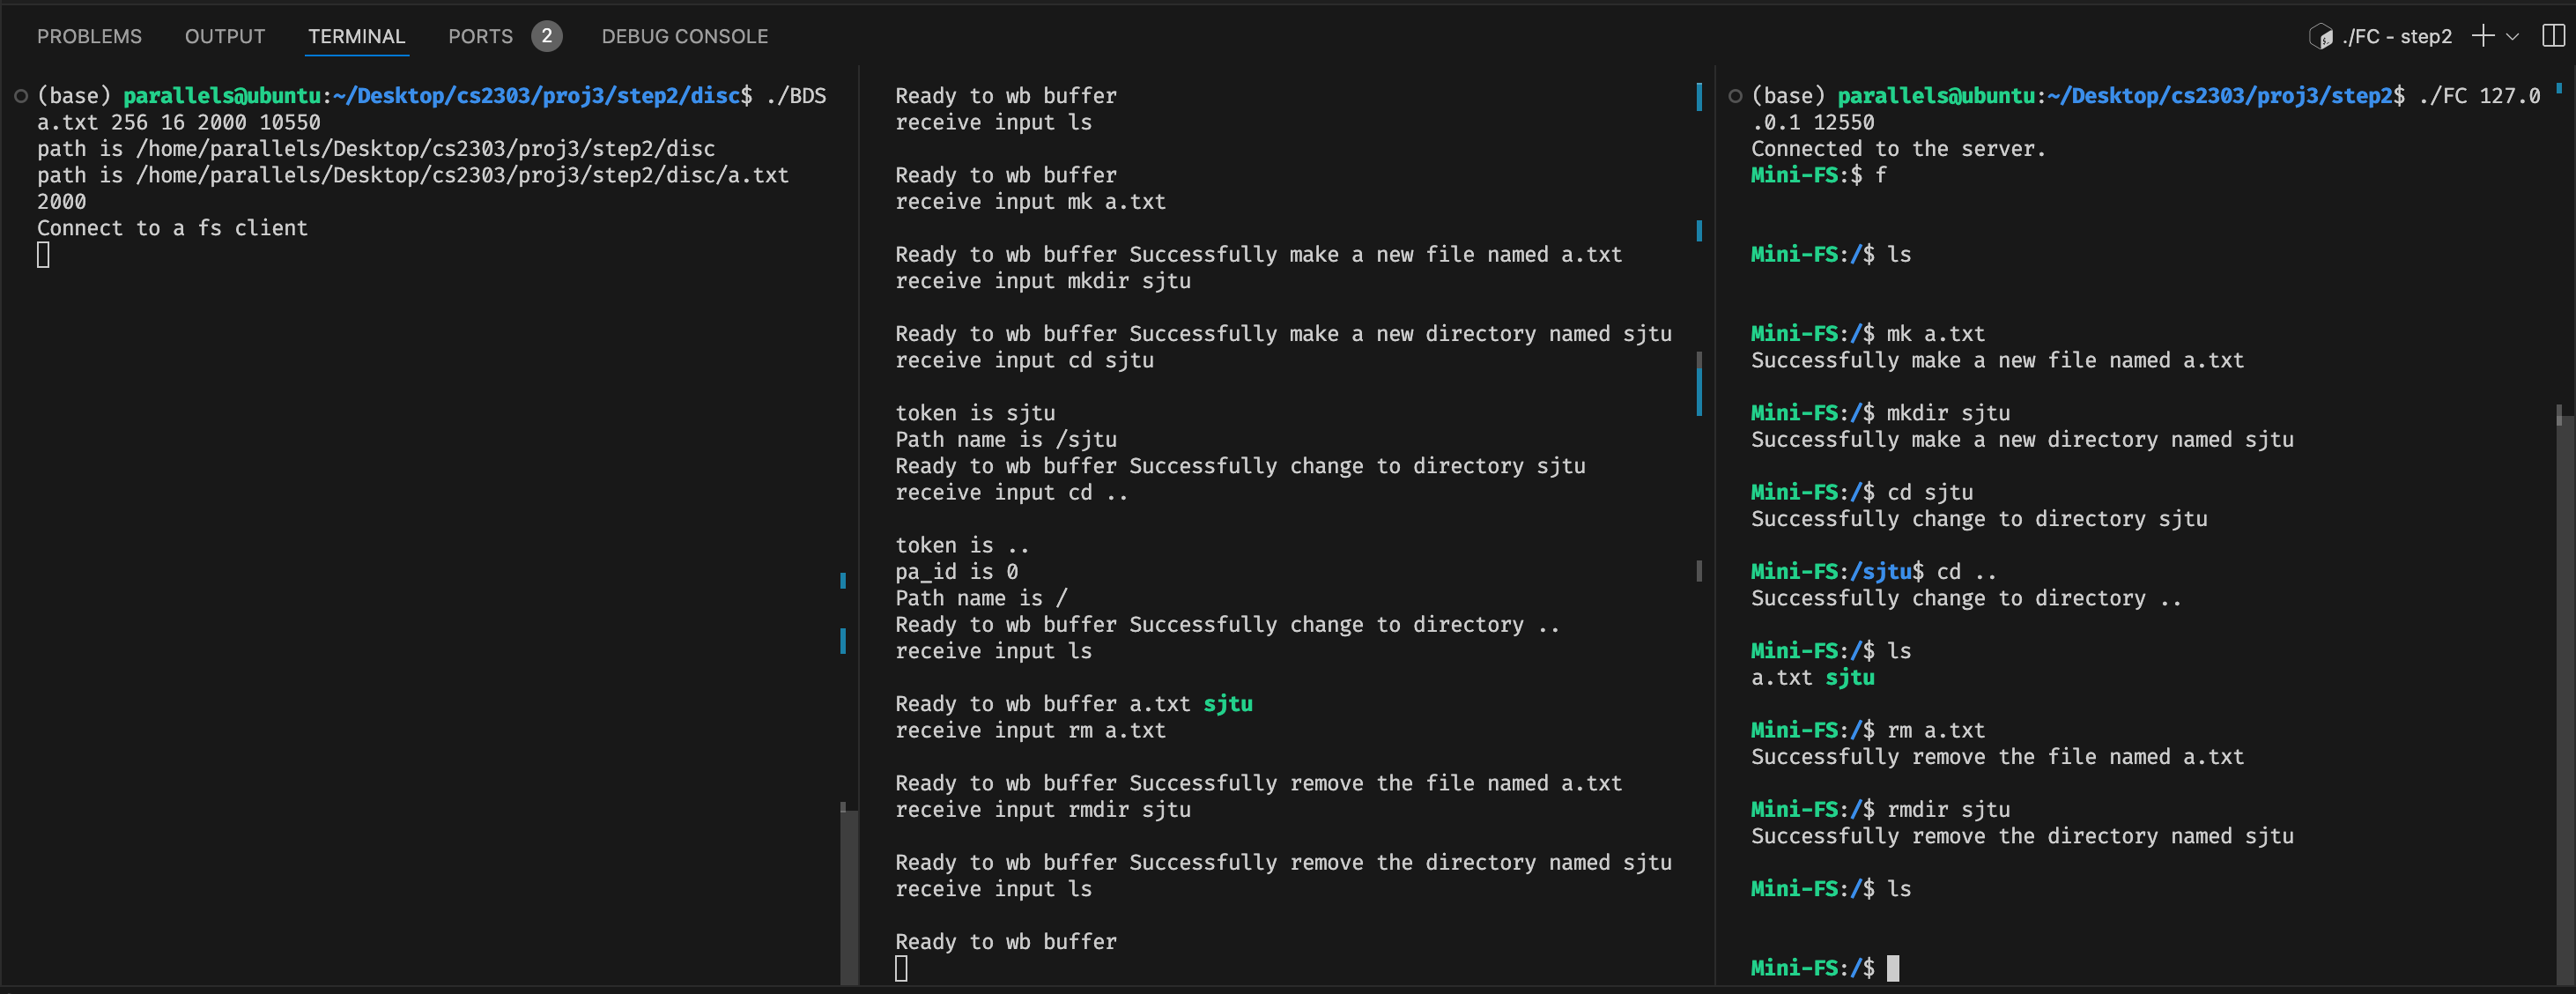
\includegraphics[width=0.8\textwidth]{fig/fc1.png}
    \caption{Result of Command line file system client Part 1.}
    \label{fig:fc1}
\end{figure}

\begin{figure}[!h]
    \centering
    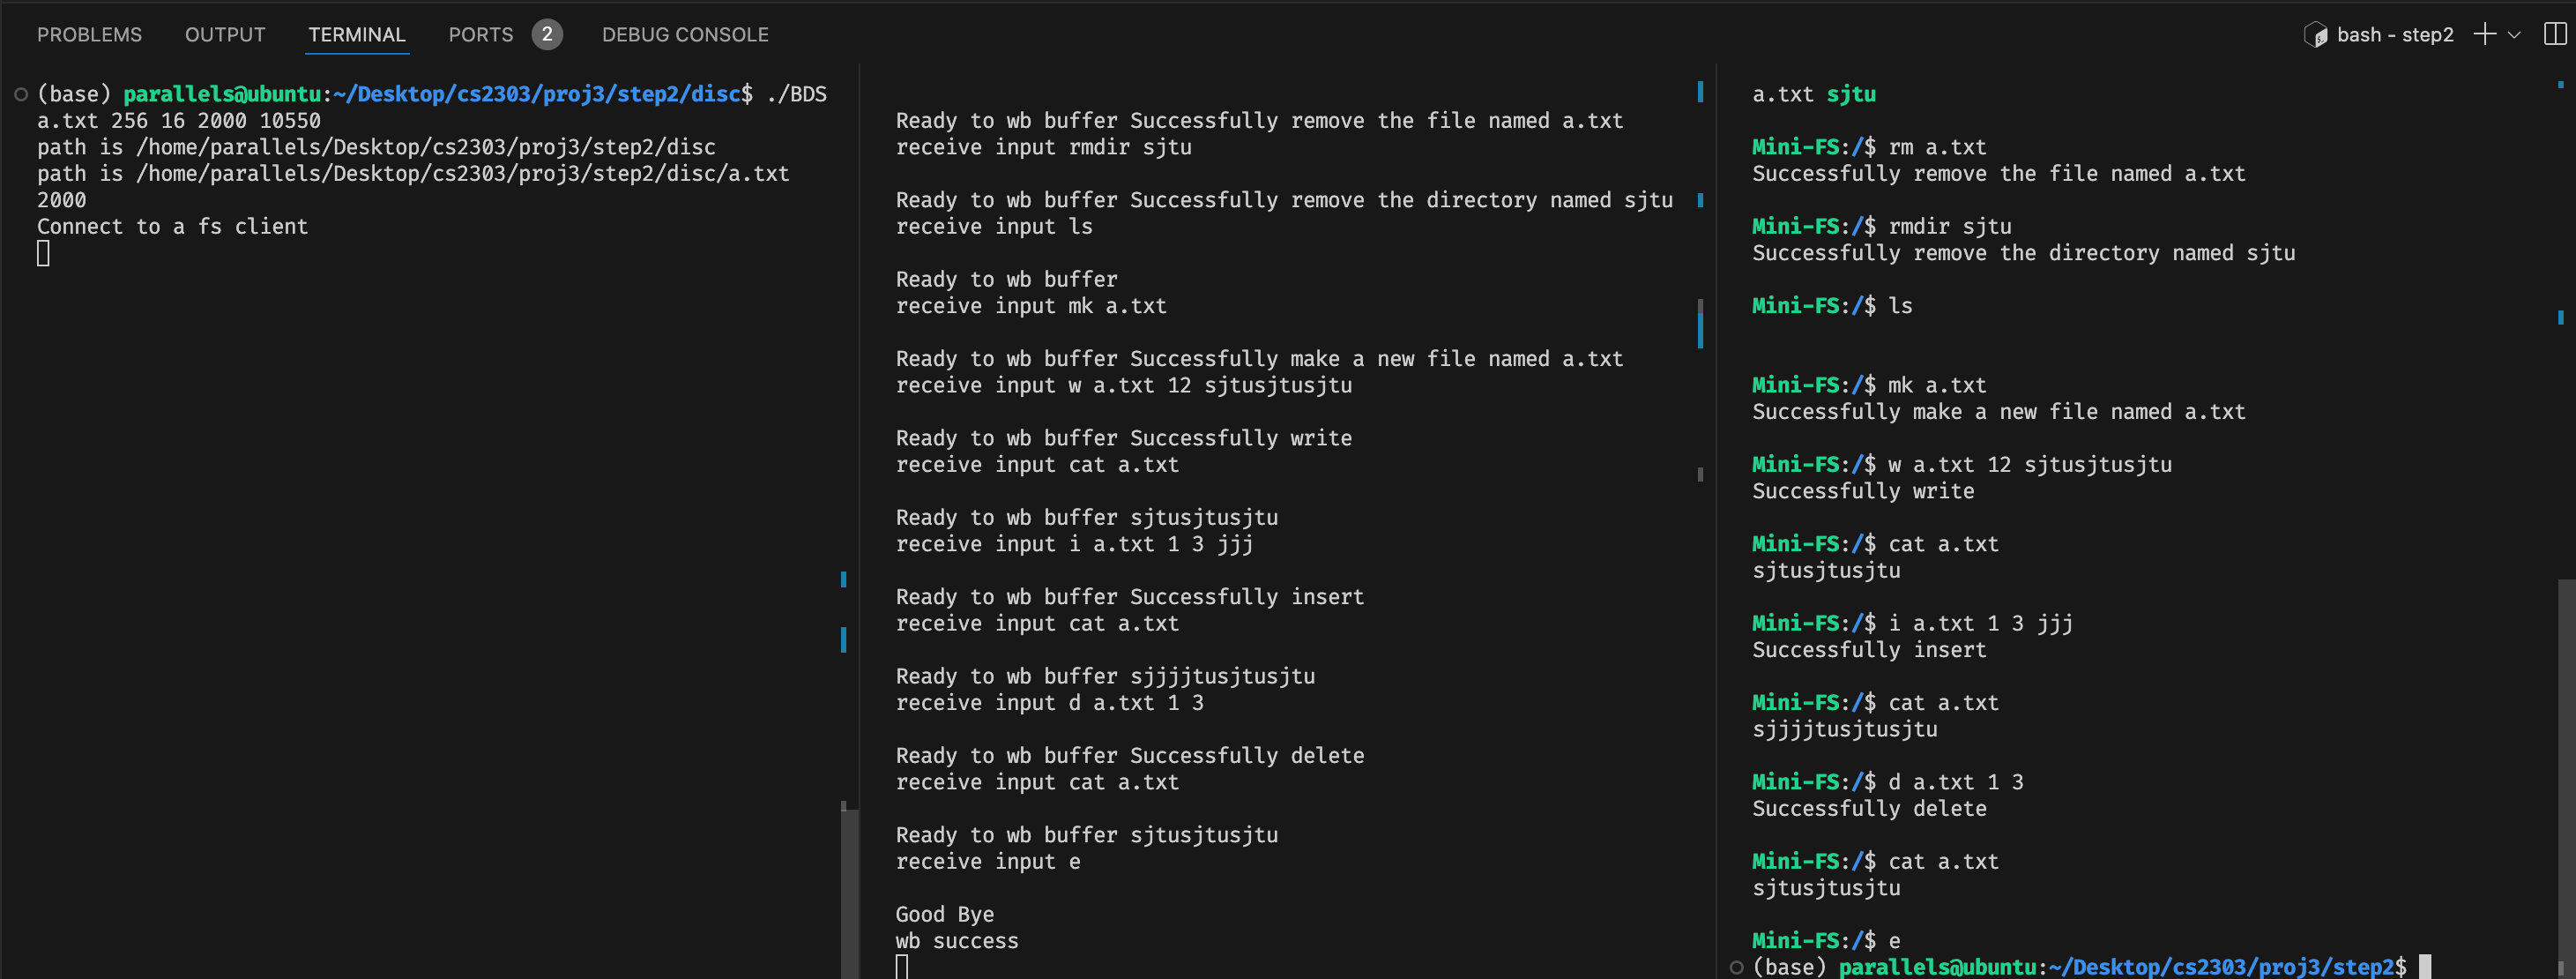
\includegraphics[width=0.8\textwidth]{fig/fc2.png}
    \caption{Result of Command line file system client Part 2.}
    \label{fig:fc2}
\end{figure}

We can easily check that our mini file system handles these commands correctly.

\section{Step 3: Support Multi-users}
In this part, we slightly modify the design of part 2 to make it support multi clients.

\textbf{Please do not use the old disc server. Instead, use the one in \texttt{proj3/step3/disc}}.

We have discussed the design of permission and ownder ID in \texttt{inode struct} in the previous part.

\subsection{User Data Structure}
In \texttt{step3/inlcude/user.h}, i design a new user data structure to store the user name and key. This is useful when we need to
create a user and login to a particular user. The struct is as follows.

\begin{lstlisting}[language=C]
    #define MAX_USER_ID 16
    #define MAX_USER_KEY 16
    
    typedef struct {
        char _user_id[MAX_USER_ID];
        char _user_key[MAX_USER_KEY];
    } User;    
\end{lstlisting}

I specially desgin the size of \texttt{\_user\_id} and \texttt{\_user\_key} to be 16, so that the size of the struct is 32.
As a result, a block can hold exactly 8 user data.

We also need to state that the index of the \texttt{_user_id} is actually the real index of the user. For example, if \texttt{\_user\_id[1]} is Jack, then 
the real index of Jack is 1. It is very useful and convenient, since we hide the index into the struct.

\subsection{Modification in \texttt{superblock.c} and \texttt{wrapper.c}}
We allow at most 6 clients including the default root client. So we need a block to store the information into. 
We select the first block after the reserve blocks, namely the \texttt{131th} block, and change the \texttt{RESERVE_BLOCK} macro from 131 to 132.

Apart from that, we add another variable \texttt{user\_count} to record how many users have been created currently.
It will be used to judge whether new users can be created.

In reality, you can see a extern global variable called \texttt{User user[8]} in \texttt{wrapper.c}, but i 
never use this variable. Every time i need to visit the user information, i directly load the 131th block into the buffer and then
use the buffer to get the user information. 

\subsection{Modification in \texttt{inode.c}}
Since we take permission into account in this part, and i set the default permission when add a new entry to be 7. Namely the owner of the 
file has read/write/execute permission, and other users do not have any permission.

The code diff is as follows.

\begin{lstlisting}[language=C]
    int dir_add_entry(Inode* inode, uint16_t clientID, char* name, uint8_t mode) {
        Entry entry[BLOCK_SIZE / sizeof(Entry)];
        // * We first check if there are vacant entry in allocated block
        int i = 0;
        for (; i < DIRECT_LINK; ++i) {
            if (inode->_direct_block[i] == 0) continue;
            // load the block into entry array
            ...
            for (int j = 0; j < BLOCK_SIZE / sizeof(Entry); ++j) {
                if (entry[j]._state == 1) continue;
                // find a new entry and do the initialization
                ...
        [PREV]      init_inode(&inode_table[inodeID], mode, 0, 0, inodeID, inode->_index, 0, clientID);
        [NOW]        init_inode(&inode_table[inodeID], mode, 0, 0, inodeID, inode->_index, 7, clientID);
                // write back
                ... 
                return 1;
            }
        }
        // * No vacant entry in allocated block
        // * Try allocate new vacant block
        i = 0;
        for (; i < DIRECT_LINK; ++i) {
            // find a vacant block and do the initialization
            ...
        [PREV]      init_inode(&inode_table[inodeID], mode, 0, 0, inodeID, inode->_index, 0, clientID);
        [NOW]        init_inode(&inode_table[inodeID], mode, 0, 0, inodeID, inode->_index, 7, clientID);
            // write back
            ...
            return 1;
        }
    }    
\end{lstlisting}

\subsection{Modification in \texttt{FS.c}}
In this file, we support 3 additional commands \texttt{cr, login, chmod}, and implement 
corresponding functions to handle these commands. I also add a \texttt{check\_permission()} function to 
check whether the current user is allowed to do the operation and then put this function to the corresponding places in the handle functions.

Since i \textbf{do not implement the optional part, namely i do not support simultaneous connection to the server}. So i do not modify the main function in \texttt{FS.c}.

There are 2 main global variables that are quite useful, \texttt{cur_inode_id and client_id}. The former is used to record the current inode id, and the latter is used to record the current user id. 
All the operations will use these 2 variables to check the permission and do the operation.

I will first expand on \texttt{cr} command. It is a command that creates a new user. The usage is \texttt{cr <user\_name> <user\_key>}. It 
enrolls a new user with given user name and user key, and update the information in the user info array stored in the 131th block in the disc.
\textbf{Note that} in my design, only the root user has the permission to create a new user and we must be at the root path to create a new user. If not, we will return an error message.
Then we will check whether the user name has been used. If it has been used, we will return an error message. If not, we will create the user and its home folder. The home folder will have the same name of the user,
and will be owned by the new user, and have the permission 7. So how to get the user id? That lies in the use of \texttt{user\_count} variable. 
After we create a new user, we will increment the \texttt{user\_count} by 1, so the id for the new user is \texttt{user\_count - 1}. 
There is another trick in the code, i change the client_id to the new user id befire \texttt{mkdirOp()} function, and then change it back to 0 after that.
That is because \texttt{mkdir()} will set the owner of the new directory to the exact value of \texttt{client_id} global variable.

The code is as follows.

\begin{lstlisting}[language=C]
    void crOp(char* name, char* key) {
        if (!initialized) {
            perror("File system not initialized.");
            return;
        }
        if (!validate_name(name)) {
            perror("Invalid name.");
            return;
        }
        memset(buffer_main, 0, MAX_BUFFER_LENGTH);
        if (cur_inode_id != 0) {
            strcat(buffer_main, "You can only create user when you are in / path");
            return;
        } 
        if (client_id != 0) {
            strcat(buffer_main, "Permission denied. cr needs super permission.");
            return;
        }
        // load the user array
        ... 
    
        if (user_count >= 6) {
            strcat(buffer_main, "Exceed maximum clients. At most 5!");
            return;
        }
    
        for (int i = 0; i < user_count; ++i) {
            if (strcmp(temp[i]._user_id, name) == 0) {
                strcat(buffer_main, "User has been created before.");
                return;
            }
        }
        
        User cur_user;
        memset(cur_user._user_id, 0, sizeof(cur_user._user_id));
        strcpy(cur_user._user_id, name);
        memset(cur_user._user_key, 0, sizeof(cur_user._user_key));
        strcpy(cur_user._user_key, key);
        // * wb
        ... 
        user_count += 1;
        client_id = user_count - 1; 

        mkdirOp(name);
        client_id = 0;
    }    
\end{lstlisting}

Then we talk about \texttt{login} command. It is a command that logs into a particular user. The usage is \texttt{login <user\_name> <user\_key>}. 
It will check whether the user name exists and whether the user key is correct. If both are correct, it will change the \texttt{client\_id} to the user id and change directory to the home directory of the user.
If not, it will return an error message. Still, we only allow to login at root path. There is another trick in the code, which is related to the shutdown of the file system server.
We know that the user array is stored in disc, so it will not be lost when the server is shut down. But the \texttt{user\_count} does not. So every time we login, we first need to count how many valid users are there in the user array and update the \texttt{user\_count} variable, then 
perform the login operation. The code is as follows.

\begin{lstlisting}[language=C]
    void login(char* name, char* key) {
        if (!initialized) {
            perror("File system not initialized.");
            return;
        }
        if (!validate_name(name)) {
            perror("Invalid name.");
            return;
        }
        if (cur_inode_id != 0) {
            strcat(buffer_main, "You can only login when you are in / path");
            return;
        }
        memset(buffer_main, 0, MAX_BUFFER_LENGTH);
        User temp[8];
        read1(sockfd, 0, 131);
        memcpy(temp, buffer[0], sizeof(temp));
        // update user count
        for (int i = 0; i < 8; ++i) {
            if (strlen(temp[i]._user_id) == 0) {
                user_count = i;
                break;
            }
        }
        // check whether the user exists
        for (int i = 0; i < user_count; ++i) {
            printf("temp id is %s, key is %s\n", temp[i]._user_id, temp[i]._user_key);
            if (strcmp(temp[i]._user_id, name) == 0 && strcmp(temp[i]._user_key, key) == 0) {
                client_id = i;
                cdOp(name);
                strcat(buffer_main, "\nSuccessfully login as ");
                strcat(buffer_main, name);
                return;
            }
        }
    }
        
\end{lstlisting}

Finally, we talk about \texttt{chmod} command. It is a command that changes the permission of a file or directory. The usage is \texttt{chmod <file\_name> <permission>}.
It will first check whether the file/directory with given name exists in the current directory inode. Then it will check whether the current client id is the owner of the file/directory or the root.
If not, it will return an error message. If yes, then it will check whether the client id has write permission to the inode, since change permission is a write operation. If yes, it will change the permission of the inode to the given permission. If not, it will return an error message. The code is as follows.

\begin{lstlisting}[language=C]
    void chmodOp(char* name, uint16_t new_perm) {
        if (!initialized) {
            perror("File system not initialized.");
            return;
        }
        if (!validate_name(name)) {
            perror("Invalid name.");
            return;
        }
        memset(buffer_main, 0, MAX_BUFFER_LENGTH);
        
        int file_inode_id = dir_check_existence(&inode_table[cur_inode_id], 0, name);
        if (file_inode_id == -1) {
            perror("File not found.");
            return;
        }
        if (client_id != 0 && inode_table[file_inode_id]._ownerID != client_id) {
            strcat(buffer_main, "Permission denied. chmod needs super permission or you need to be the owner.");
            return;
        }
    
        if (check_permission(2, file_inode_id) == 0) {
            strcat(buffer_main, "Permission denied. chmod needs write permission.");
            return;
        }
        inode_table[file_inode_id]._permission = new_perm;
        strcat(buffer_main, "Successfully change the permission of ");
        strcat(buffer_main, name);
        write_inode_to_disc(&inode_table[file_inode_id], client_id, file_inode_id);
    }    
\end{lstlisting}

Then let's look at how \texttt{check\_permission()} function works. It checks whether the current client id has enough permission to visit a particular inode id.
If the current client is root, we just return 1 since root has super permission. Then if the current client is the owner of the inode, we check the low 3 bits of the permission and the mask provided as parameter. If any bit of the mask is 1 and the corresponding bit of the permission is 0, we return 0, otherwise we return 1. 
If the current client is not the owner of the inode, we check the 3rd to 5th bits of the permission and the mask provided as parameter. If any bit of the mask is 1 and the corresponding bit of the permission is 0, we return 0, otherwise we return 1. 

We should provide the permission mask based on the operation as parameter. Detailed permission will be discussed later. The code is as follows.

\begin{lstlisting}[language=C]
    int check_permission(uint16_t mask, int inode_id_cur) {
        if (client_id == 0) {
            // * root has super permission
            return 1;
        }
    
        uint16_t perm = inode_table[inode_id_cur]._permission;
        uint16_t indx = inode_table[inode_id_cur]._ownerID;
        uint16_t read_mask = mask & (1 << 2);
        uint16_t write_mask = mask & (1 << 1);
        uint16_t exec_mask = mask & 1;
        if (indx == client_id) {
            if (read_mask && !(perm & (1 << 2))) {
                return 0;
            }
            if (write_mask && !(perm & (1 << 1))) {
                return 0;
            }
            if (exec_mask && !(perm & (1 << 0))) {
                return 0;
            }
        } else {
            if (read_mask && !(perm & (1 << 5))) {
                return 0;
            }
            if (write_mask && !(perm & (1 << 4))) {
                return 0;
            }
            if (exec_mask && !(perm & (1 << 3))) {
                return 0;
            }
        }
        return 1;
    }    
\end{lstlisting}

Finally, let's look at the commands we support need what permission respectively.
\begin{itemize}
    \item \texttt{f} command does not need permission, since in part 3, the file system server will initialize automatically.
    \item \texttt{ls} command needs read permission, so the mask is 4 (0b100).
    \item \texttt{e} command does not need permission, since it is just an exit command.
    \item \texttt{mk} command needs write and exec permission, so the mask is 3 (0b011).
    \item \texttt{mkdir} command needs write and exec permission, so the mask is 3 (0b011).
    \item \texttt{rm} command needs write permission, so the mask is 2 (0b010).
    \item \texttt{rmdir} command needs write and exec permission, so the mask is 3 (0b011).
    \item \texttt{cat} command needs read permission, so the mask is 4 (0b100).
    \item \texttt{w} command needs write permission, so the mask is 2 (0b010).
    \item \texttt{i} command needs read and write permission, so the mask is 6 (0b110).
    \item \texttt{d} command needs read and write permission, so the mask is 6 (0b110).
    \item \texttt{cd} command in my design do not need permission, since it is just a change directory operation.
\end{itemize}

If the current client id does not have enough permission, then he is not allowed to perform that operation.
User can manually change the permission of his own file via \texttt{chmod} command to share with other users.

\subsection{Result Demo}
The basic read/write operation is the same with step 2, so we focus on showing the new commands in this part. 

Check Fig~\ref{fig:p1} and Fig~\ref{fig:p2}.

\begin{figure}[!h]
    \centering
    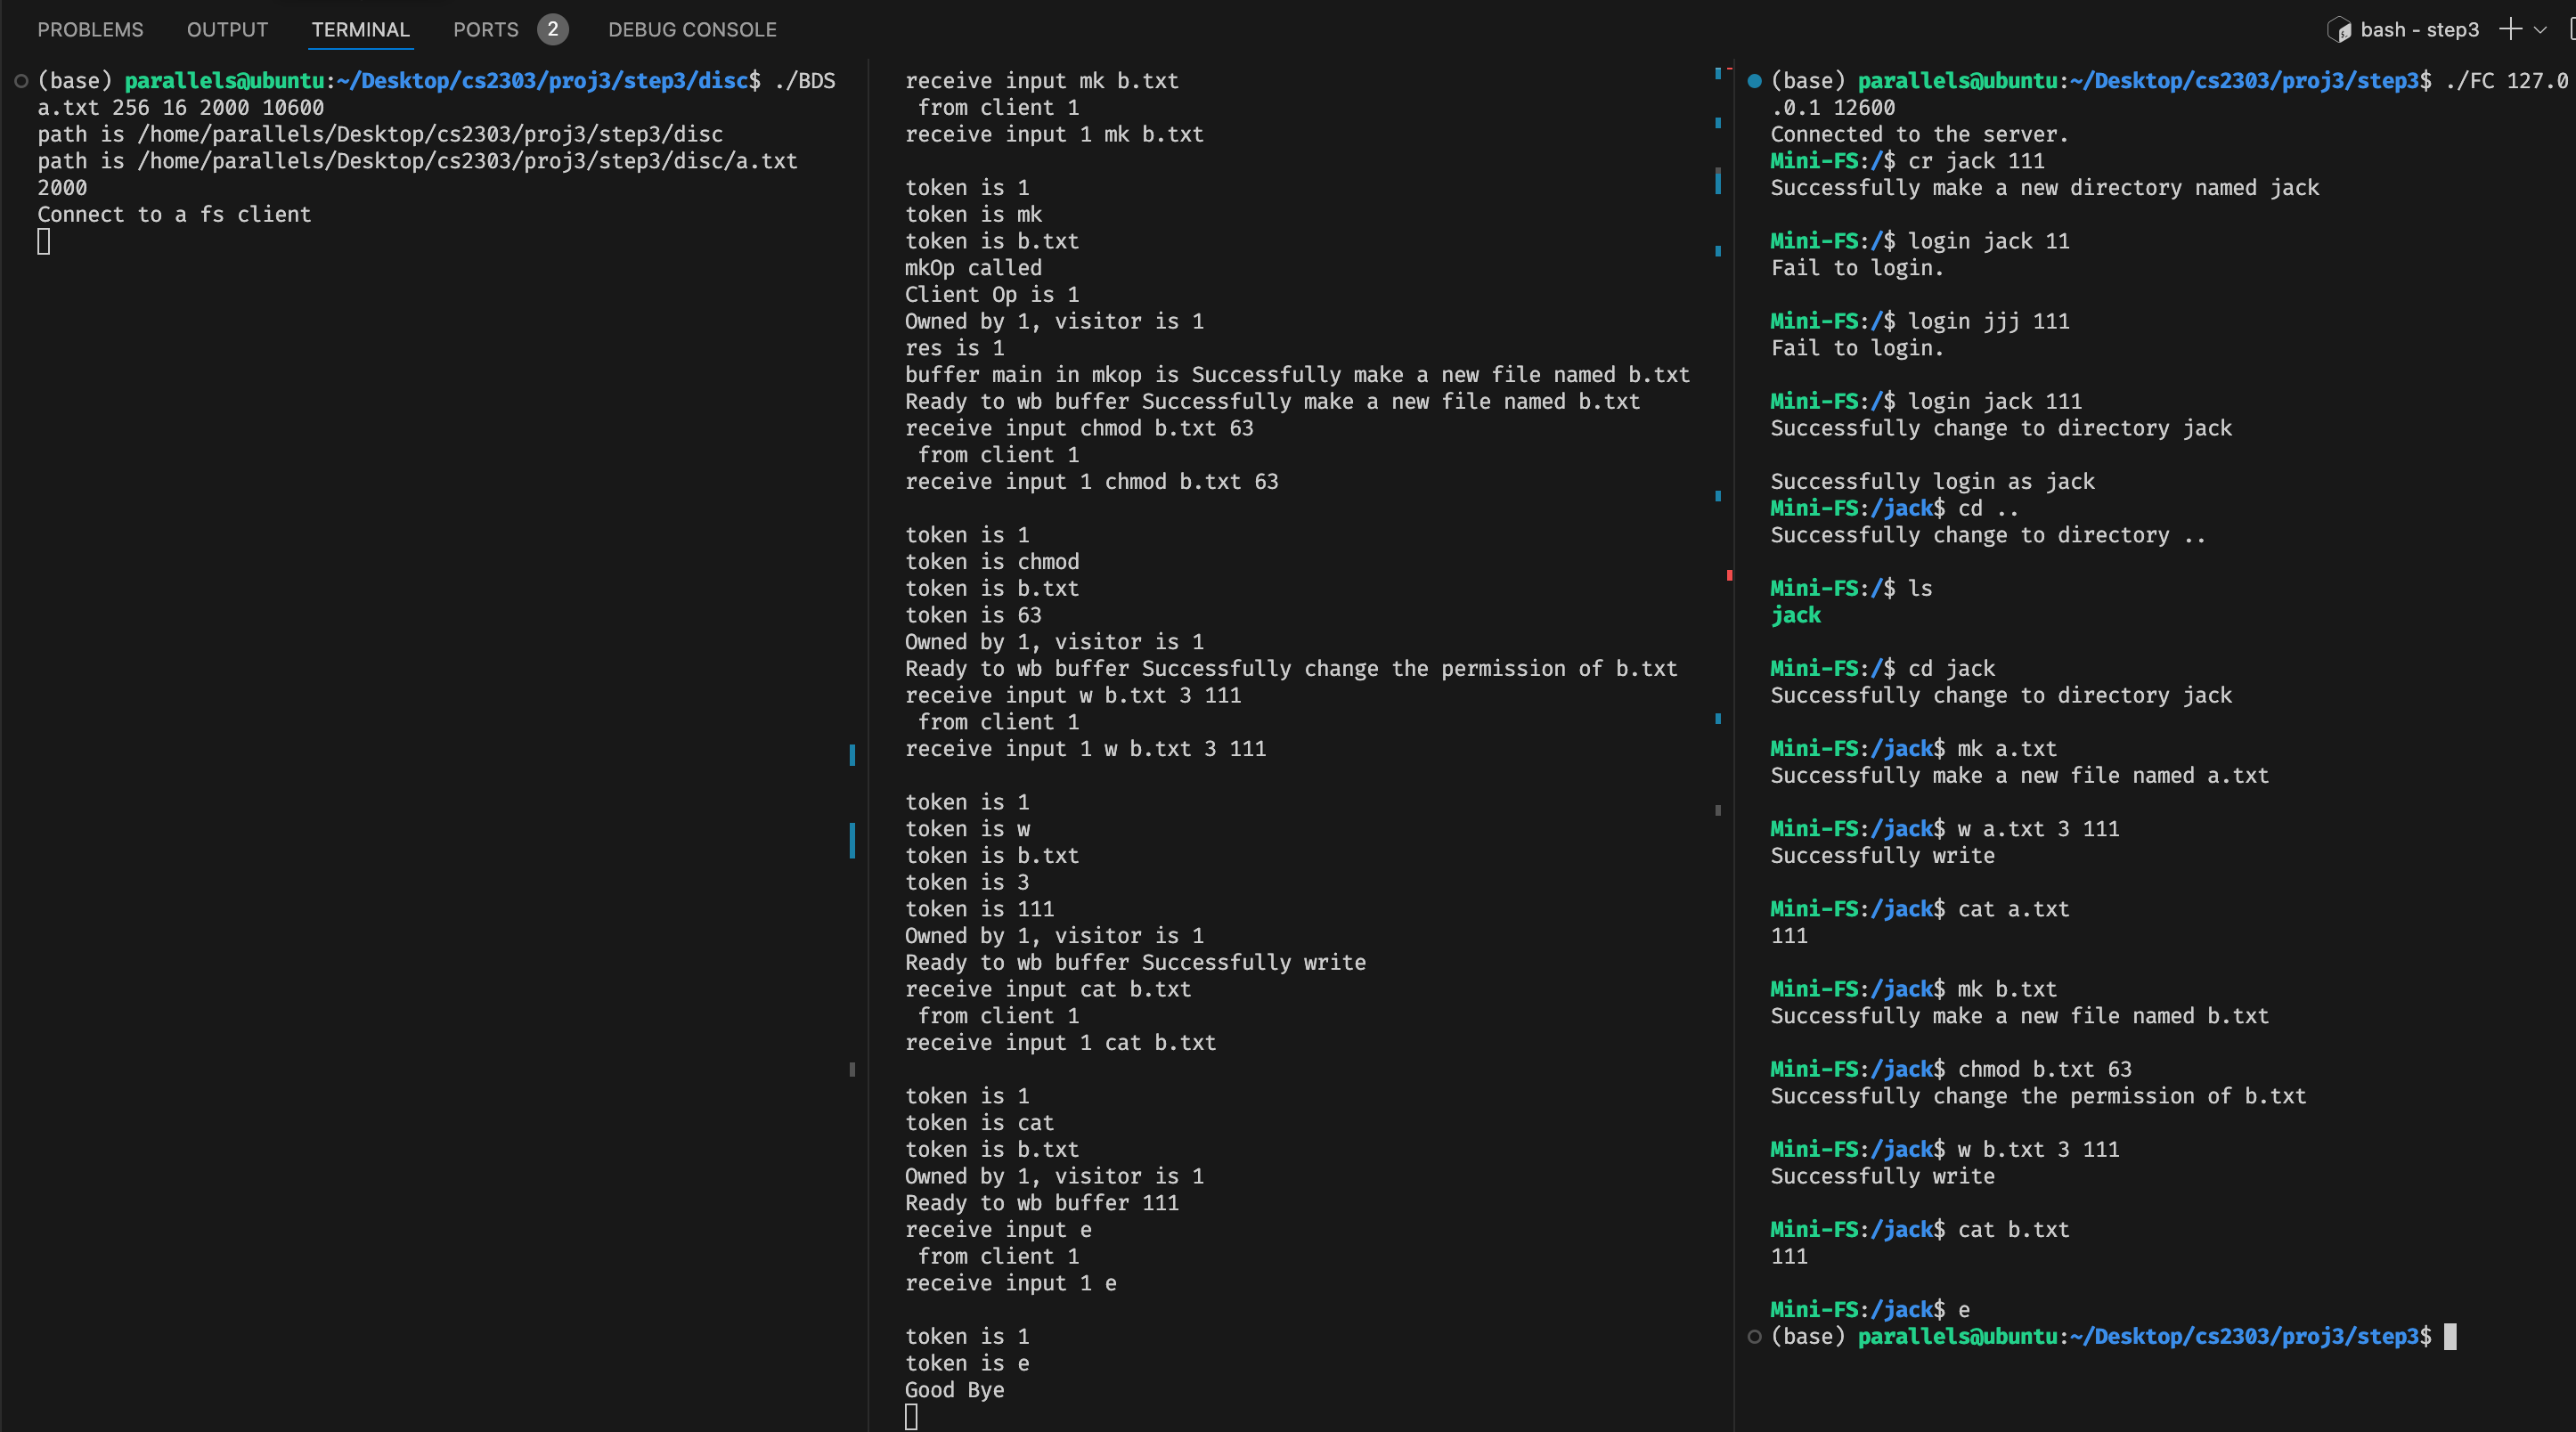
\includegraphics[width=0.8\textwidth]{fig/p1.png}
    \caption{Result of Part 3 Command line test 1.}
    \label{fig:p1}
\end{figure}

\begin{figure}[!h]
    \centering
    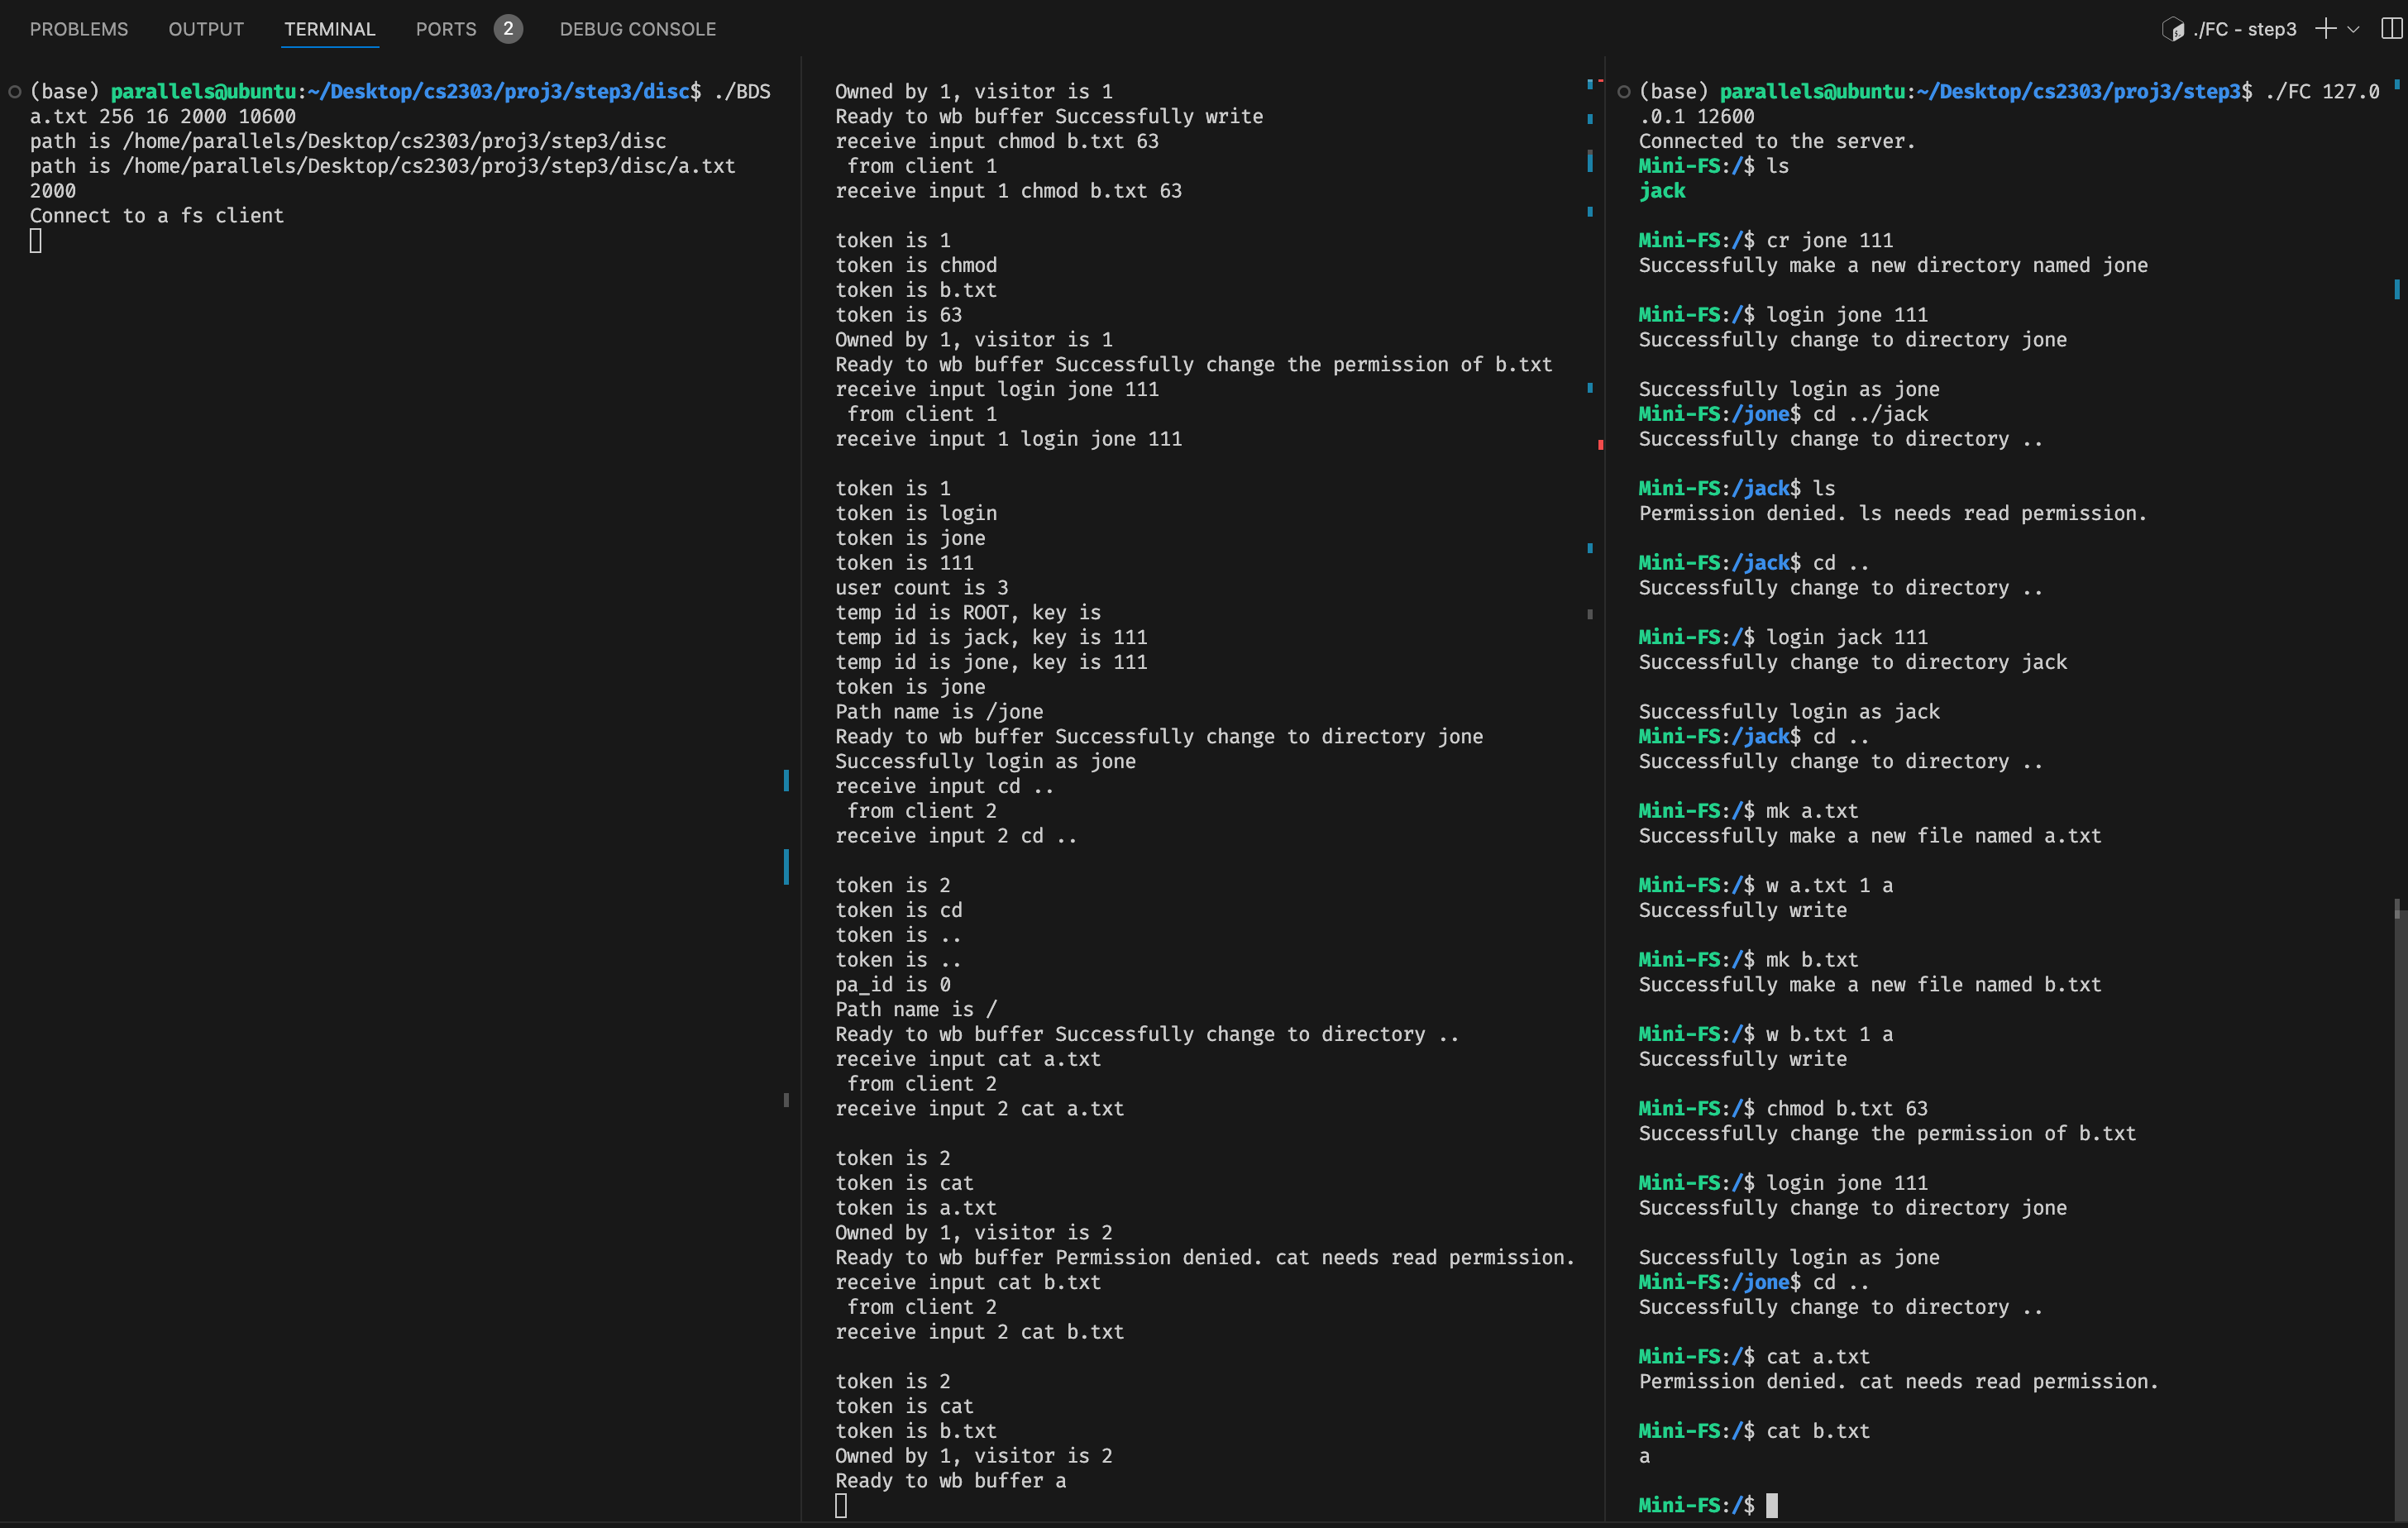
\includegraphics[width=0.8\textwidth]{fig/p2.png}
    \caption{Result of Part 3 Command line test 2.}
    \label{fig:p2}
\end{figure}

In Fig~\ref{fig:p1}, we can see that we first create a new user called \texttt{jack}, and try 
to login with wrong name and key, the server throws error correctly. After that, we correctly login to the user \texttt{jack} and the current path 
changes to the home folder correctly. And then we make two txt files and test the \texttt{chmod} command. 

In Fig~\ref{fig:p2}, we create another user called \texttt{jone}, and login to it. We then cd to jack's home folder and try to \texttt{ls}, which throws error since we do not have permission. 
Then we change the permission of the file \texttt{test.txt} to 6, and then we can \texttt{ls} successfully.
We then login to \texttt{jack}, and create two txt file in the root path, one with the permission for other users to read via \texttt{chmod b.txt 63}, and one without.
We then login to \texttt{jone} and try to \texttt{cat} the two files, and we can see that we can only read the file \texttt{b.txt}. That indicates that the permission system works correctly.

\section{Summary}
In this project, we develop a file system based on socket communication. We progressively design a disc simulator, a file system server and a file system client. At last we modify the file system
server to support multi-clients.

During the development, i gain a better understanding of how the file system works, and learns about the real linux ex2 file system.
Apart from that, i have a better understanding of C language and socket communication. C is quite a powerful language, and supports direct interation with the hardware, which is quite useful in system programming.
But the poor string manipulation really makes me feel bad. I consider refactor the code in modern C++ or Rust to have a play. 
I also practise module design in this project, separating header file from source file. I do think that a clear API and abstraction really helps our design.

Thanks the teacher Li and TAs for their hard work in this course. I really learn a lot from this course.